\documentclass[10pt,a4paper]{article}


\usepackage[T1]{fontenc}
% \usepackage[utf8]{inputenc}
\usepackage[english]{babel}
\usepackage[english]{isodate}
\usepackage[parfill]{parskip}
\usepackage[margin=3.cm]{geometry}
\usepackage{graphicx}
\graphicspath{{./figs/}}
\usepackage{amsmath}
\usepackage{amssymb}
%\usepackage{cite}
\usepackage{array}
\usepackage{natbib}
\usepackage[caption=false]{subfig}
\usepackage{titling}
\usepackage{titlesec}

\usepackage{xcolor}

\definecolor{bcolor}{rgb}{0.95,0.95,1.0}

\usepackage[caption=false]{subfig}
\usepackage{caption}
%\usepackage{orcidlink}
\usepackage{hyperref}
\hypersetup{
	colorlinks = true,
	urlcolor   = blue,
	citecolor  = blue,
	linkcolor = blue
}

\title{\Huge \sffamily \textsc{\textbf{User Manual}}}
\author{}%Ron Shnapp}
\date{}



\pretitle{%
	\begin{center}
		\LARGE
		
\includegraphics[width=8cm]{logo.png}\\[3cm]
	}
\posttitle{\end{center}}


\begin{document}
	
	


	
\maketitle

\thispagestyle{empty}
\vspace{2.5cm}

\begin{center}
	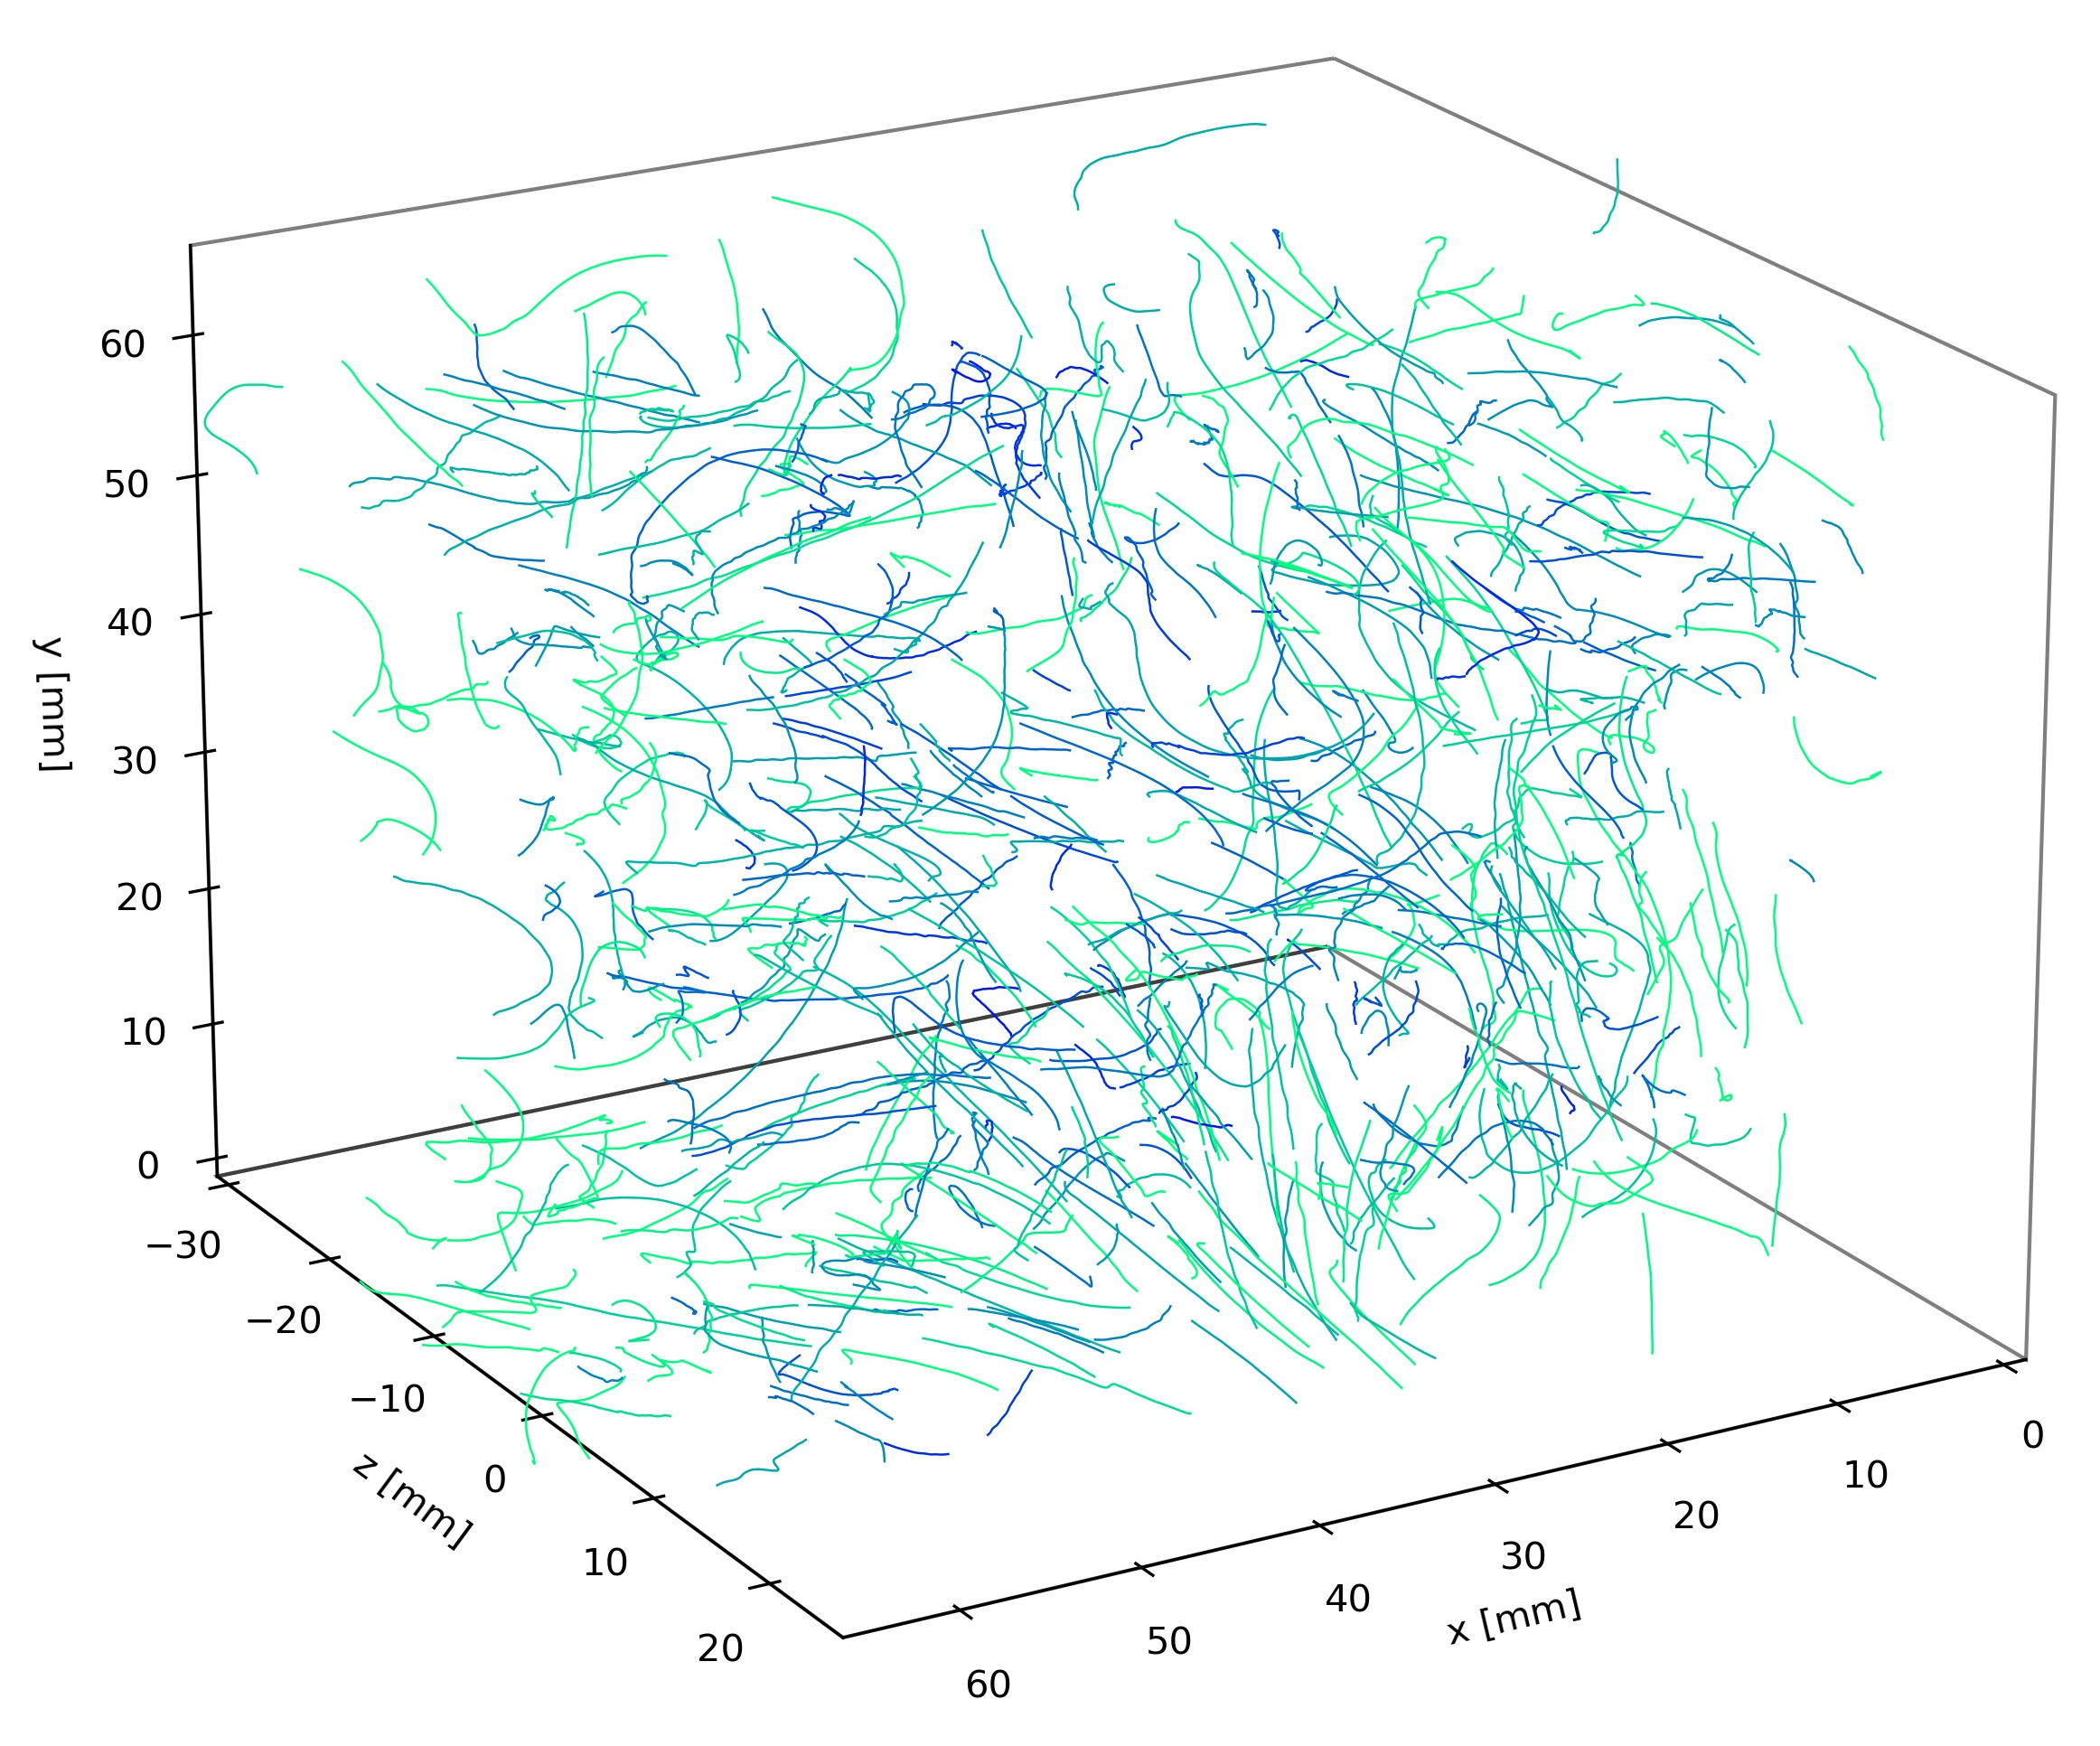
\includegraphics[width=10cm]{traj_image.jpg}
\end{center}

\vfill

\begin{minipage}{14cm}
	{\small \sffamily
	Vesrion: 0.6.0 \\
	Last updated: \today \\
	Github repository: \url{https://github.com/ronshnapp/MyPTV} \\
	Get help \& interact with our community: \url{https://github.com/ronshnapp/MyPTV/discussions}\\
	Contact the developers: ronshnapp@gmail.com}
\end{minipage}



\newpage
% ================================
%            TOC
% ================================
\tableofcontents
\pagenumbering{Roman}
\newpage

\pagenumbering{arabic}








% ================================
%            Section 1
% ================================


\section{Introduction}

\subsection{3D-PTV principles}


The 3D-PTV method is used to measure the trajectories of particles in 3D space. It utilizes the principles of stereoscopic vision to reconstruct 3D positions of particles from images taken from several angles. A scheme of a typical 3D-PTV experiment using a four-camera system is shown in Fig.~\ref{fig:3dptv_exp}. The "workhorse" behind the 3D-PTV method is the co-linearity condition, the 3D model. In principle, if we know what the position is and what is the orientation of the camera in 3D space ($O'$ and $\theta$ in Fig.~\ref{fig:3dmodel}), we can use the pin-hole camera model to relate the image space coordinates of a particle ($\eta,\, \zeta$ in Fig.~\ref{fig:3dmodel}) to the ray of light connecting the imaging center and the particle. Then, if we have more than one camera, the particle will be located at the intersection of the two rays. Detailed information is given in \cite{Virant1997, Maas1993}.  


\begin{figure}[!ht]
	\centering
	\subfloat[]{\label{fig:3dptv_exp}
		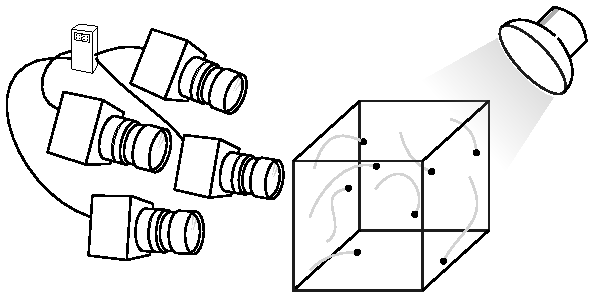
\includegraphics[width=6.5cm]{3D_PTV_acquisition.pdf}}
	\hfill
	%
	\subfloat[]{\label{fig:3dmodel}
		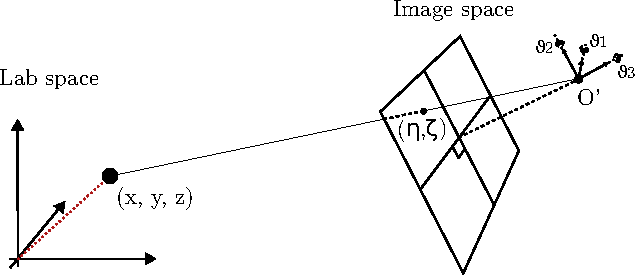
\includegraphics[width=6.5cm]{pinhole_model.pdf}}
	%
	\caption{(a) A schematics of a 3D-PTV experiment. (b) A schematic description of the 3d model, the pin-hole camera model.}
\end{figure}



Once the experiment, namely data acquisition, is done, there are six intrinsic steps to follow in order to complete the analysis. The six steps are outlined in Fig.~\ref{fig:steps}. In the camera calibration step, we use images of known calibration targets to estimate the position, orientation, and internal parameters of the cameras. In particle segmentation, we use image analysis to obtain the particles' image space coordinates ($\eta, \, \zeta$). In the Particle matching step, we use the ray crossing principle to decide which particle image in each camera corresponds to the same physical particle, and triangulate their positions through stereo matching. In particle tracking, we connect the positions of particles in 3D space to form trajectories. In data conditioning, we might use smoothing and re-tracking algorithms to enhance our data quality according to some physical heuristics. Lastly, we can analyze the data to obtain information on the physics of the particles we are studying. The MyPTV package is meant to handle the first five of these steps.    



\begin{figure}
	\centering
	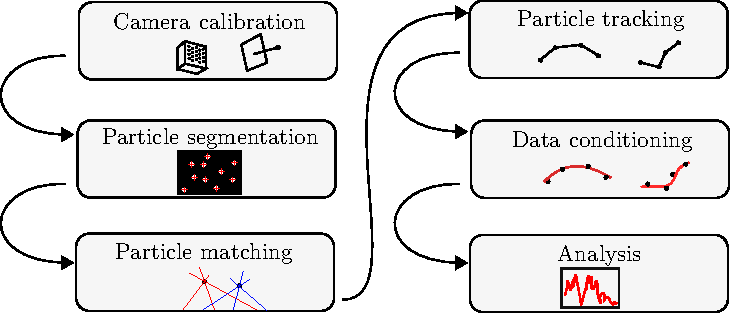
\includegraphics[width=10cm]{steps.pdf}
	\caption{Basic steps in the analysis of PTV raw data into particle trajectories and scientific output. The first five steps are handled by MyPYV. \label{fig:steps}}
\end{figure}


The sections that follow outline the code used to handle the 3D-PTV method in MyPTV.





\subsection{3D model}


We use a pinhole camera model to transform the 2D particles seen in the camera images. In particular, the following expression relates the coordinates in the 2D image space coordinates and a direction vector pointing out from the camera imaging center:
%
\begin{equation}
\vec{r}-\vec{O} = \Big( \, 
\begin{bmatrix}
\eta + x_h\\
\zeta + y_h \\
f
\end{bmatrix}
+ \vec{e}(\eta, \zeta) \,\Big) \cdot \Big[ R \Big]
\label{eq:3dmodel}
\end{equation}
%
where the description of the notations is given in Table~\ref{tab1:mathdesc}. The matrix $[R]= [R_1]\cdot [R_2] \cdot [R_3]$ is the rotation matrix calculated with the components of the orientation vector, $\vec{\theta} = [\theta 1,\, \theta 2,\, \theta 3]$. In addition, the correction term $\vec{e}$ is assumed to be a quadratic polynomial of the image space coordinates:
%
\begin{equation}
\vec{e}(\eta,\,\zeta) = [E]\cdot P(\eta,\,\zeta) =
\begin{bmatrix}
E_{11} & E_{12} & E_{13} & E_{14} & E_{15}\\
E_{21} & E_{22} & E_{23} & E_{24} & E_{25}\\
0 & 0 & 0 & 0 & 0
\end{bmatrix}
\cdot 
\begin{bmatrix}
\eta\\
\zeta\\
\eta^2\\
\zeta^2\\
\eta\,\zeta
\end{bmatrix}
\end{equation}
%
where $[E]$ is a $3\times5$ matrix that holds the correction coefficients; the last row is filled with zeros because we do not attempt to correct $f$.





\begin{table}[!ht]
	\centering
	\caption{Description of mathematical notation. \label{tab1:mathdesc}}
	\begin{tabular}{p{5em} p{30em}}
		\hline
		Symbol & Description \\ \hline
		$\vec{r}$ & Particle position in the lab space coordinates\\
		$\vec{O} $& Position of a camera's imaging center \\
		$\eta, \, \zeta$ & image space coordinates (pixels) of a particle \\
		$x_h , \, y_h$ & Correction to the camera's imaging center (in pixels)\\
		$f$ & The camera's principle distance divided by the pixel size \\ 
		$\vec{e}(\eta, \zeta)$ & A nonlinear correction term to compensate for image distortion and multimedia problems.\\
		$[R]$ & The rotation matrix which corresponds to the camera orientation vector. \\  \hline
	\end{tabular}
\end{table}















\subsection{MyPTV usage and structure}


MyPTV is used to conduct the post-processing steps in which the experimental raw data (images) are transformed into particles' trajectories. The five steps include camera calibration, image segmentation, particle matching, particle tracking, and, data conditioning which is divided into smoothing and stitching of broken trajectories. This section outlines how these steps are to be followed and how MyPTV is structured to facilitate them. Section~\ref{sec:workflow} gives instructions on how to efficiently use MyPTV. 


At the current stage, MyPTV does not include a graphical user interface. Instead, the package includes a script that can be used to efficiently and conveniently run the various post-processing steps. Knowledge of Python is not required to operate MyPTV.


The internal structure of MyPTV is made of separate "modules", each of which deals with a particular step out of the list described above. Each module consists of a Python script file that includes one or several classes. Detailed information on each of these classes is given in Sections~\ref{sec:image_mod}--\ref{sec:stitching}, and the code itself includes documentation to a level appropriate for development. In addition to the source code, MyPTV includes a \textit{workflow} script that is used to operate the software in an organized fashion. Thus, MyPTV can be used either by using the workflow script or by directly evoking classes from the source code. 







\clearpage



\section{The Workflow: guidelines for a 3D-PTV experiment}\label{sec:workflow}


MyPTV can be operated using the \texttt{workflow.py} script. The script is found under the \textit{example} folder under the home directory of the MyPTV package. The workflow is used through command line given instructions and a file that outlines the parameters to be used in each step.





\subsection{Preparation of an experiment folder}~\label{sec:workflow_exp_folder}

To begin post processing of the 3D-PTV results, prepare the following directory structure:

\begin{enumerate}
	\item Make a new directory; in it, make a new directory called \texttt{Calibration} and place inside it the calibration images, and make another set of directories, one for each camera, and place inside it the particle images of each camera.
	\item Locate the \texttt{example} under the root folder of the MyPTV package. This can be used as a template to the experiment directory made in the previous step.
	\item Copy the files \texttt{workflow.py} and \texttt{params\_file.yml} from the \texttt{example} folder into your experiment's folder.
\end{enumerate}




\subsubsection{The \texttt{workflow.py} script} \label{sec:workflow_commands}

\texttt{workflow.py} is a Python script used by the user to run the various steps of the post-processing. The script is used through the terminal or command line. To use MyPTV's various functions, go to the experiment's directory with:
\begin{verbatim}
cd \path\to\experiment\folder
\end{verbatim}
%
and then, use the following syntax:
%
\begin{verbatim}
python workflow.py params_file.yml "command"
\end{verbatim}
%
where \texttt{"command"} should be replaced with one of the following options, depending on the particular step of the post processing:
%
\begin{verbatim}
	help
	initial_calibration
	final_calibration
	calibration_with_particles
	segmentation
	matching
	tracking	
	smoothing
	stitching
	2D_tracking
\end{verbatim}
%
Each of these commands initiates one of MyPTVs functionalities, and a detailed explanation on them is found in Sections \ref{sec:cal_guide}--\ref{sec:workflow_stitch}. Use \texttt{help} to print the available list of commands.


\subsubsection{The \texttt{params\_file.yml} file}

The \texttt{params\_file.yml} outlines all the parameters needed in order to run MyPTV using the workflow script. In every step conducted, go through the lists of parameters and make sure that their values are correct. The definitions per every step are tabulated in the sections below.







\subsection{Calibration guide} \label{sec:cal_guide}


A good calibration is key to having success in your PTV experiment! Thus, follow this guide to calibrate your camera using MyPTV. 


In the process called camera calibration, our goal is to determine what are the external ($\vec{O}$, $\vec{\theta}$) and internal ($f$, $x_h,\,y_h$, $[E]$) parameters of each of our cameras. This process is done by taking an image, a \textit{calibration image}, of an object that has points with known coordinates marked on it - \textit{calibration target}. Therefore, its important to make sure that for each experiment and each camera we have a calibration image ready, as seen, for example, in Fig.~\ref{fig:cal_img}.


Importantly, since our goal in calibration is to find the cameras' positions, once calibration images were taken in an experiment it is crucial that the cameras are not moved. Even minor vibrations can ruin an experiment. Also, the calibration target needs to be in the same medium in which the experiment will be performed to ensure that any refraction is corrected by the error terms (for example, if you are using a tank of water, place the calibration target inside the tank of water). 


The calibration in MyPTV is performed in two steps: \textit{initial calibration} and \textit{final calibration}. The initial calibration is used to obtain a rough estimation of some of the camera's parameters using a small number of calibration points, as well as to extract the information for all the calibration points on the calibration target. In the final calibration we fine tune the camera's parameters in order to minimize the \textit{calibration error}. The process is explained in detail in the following sub sections. 


%A schematic block diagram for the calibration process of each camera is given in Fig.~\ref{fig:calibsteps}. The calibration is divided into two sub-processes: 1) initial calibration, in which we use only 6 calibration points to obtain an approximate calibration estimation, and, 2) final calibration, in which we use all the calibration points on the calibration target to improve the accuracy of the initial calibration. The various steps of the process are performed in MyPTV through the workflow script, and detailed instructions are given below. 
%
%
%\begin{figure}
%	\centering
%	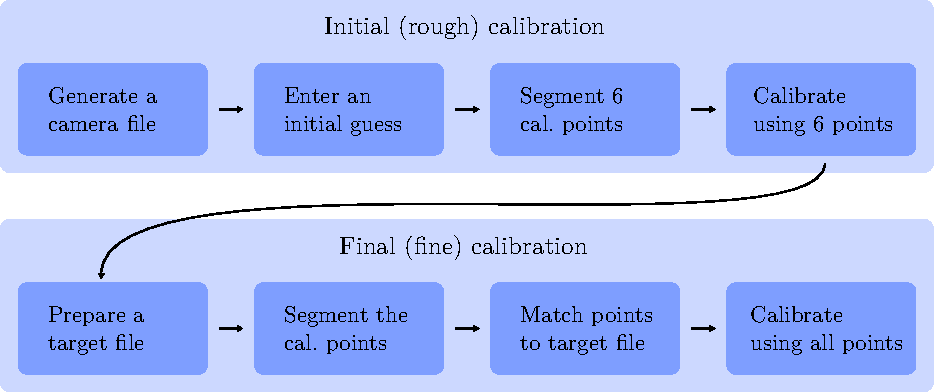
\includegraphics[width=10cm]{Calibration_steps.pdf}
%	\caption{A block diagram representing the steps to follow in the calibration of each camera using MyPTV. \label{fig:calibsteps}}
%\end{figure}




\subsubsection{Preparing a \texttt{target\_file}}

The target file is a text file (tab separated values), in which each row shows the lab space coordinates of a calibration point.  An example for the format is shown in Fig.~\ref{fig:target_file}. If there is no target file in the experimental folder, this is the time to generate one. Prepare such a file and save it in the experiment's calibration folder.




\subsubsection{Preparing the parameters in the \texttt{params\_file}}

As in any step of MyPTV, we make sure that the \texttt{params\_file.yaml} in our experiment folder has the correct parameters, namely file names under the calibration tab; see Tab.~\ref{tab:cal_paramsfile}. Each camera is calibrated separately, and so, for the calibration of each camera we need to change the file names in \texttt{params\_file.yaml} appropriately (alternatively, one could have separate parameter files for each camera).  

\begin{table}
	\centering
	\caption{The \texttt{params\_file.yml} parameters for the calibration step. All paths to files are relative to the \texttt{workflow.py} script. \label{tab:cal_paramsfile}}
	\begin{tabular}{l m{10cm}}
		\hline
		Parameter & Description\\
		\hline
		\texttt{camera\_name} & the name of the camera to be calibrated; for example, \texttt{cam1}, etc. \\
		
		%\texttt{calibration\_points\_file} & path to the file that lists the correlated lab space and image space coordinates \\
		
		\texttt{target\_file} & path to the file that lists the calibration target's lab points \\
		
		%\texttt{segmented\_points\_file} & path of the file with segmented calibration points \\
		
		\texttt{calibration\_image} & path of the calibration image \\
		
		\texttt{resolution} & camera resolution; for example: 1280, 1024\\
		\hline
	\end{tabular}
\end{table}





\subsubsection{Initial calibration}\label{sec:init_calibration}


To start the initial calibration, we start the \textit{initial calibration GUI}. Using the workflow file in the terminal, use the following command:
%
\begin{verbatim}
python workflow.py params_file.yml initial_calibration
\end{verbatim} 
%
which should open the a window like the one shown in Fig.~\ref{fig:init_cal_gui}. The left most panel shows the calibration image; we can zoom in and out by pressing the "+" and "-" keys. 

\begin{figure}
	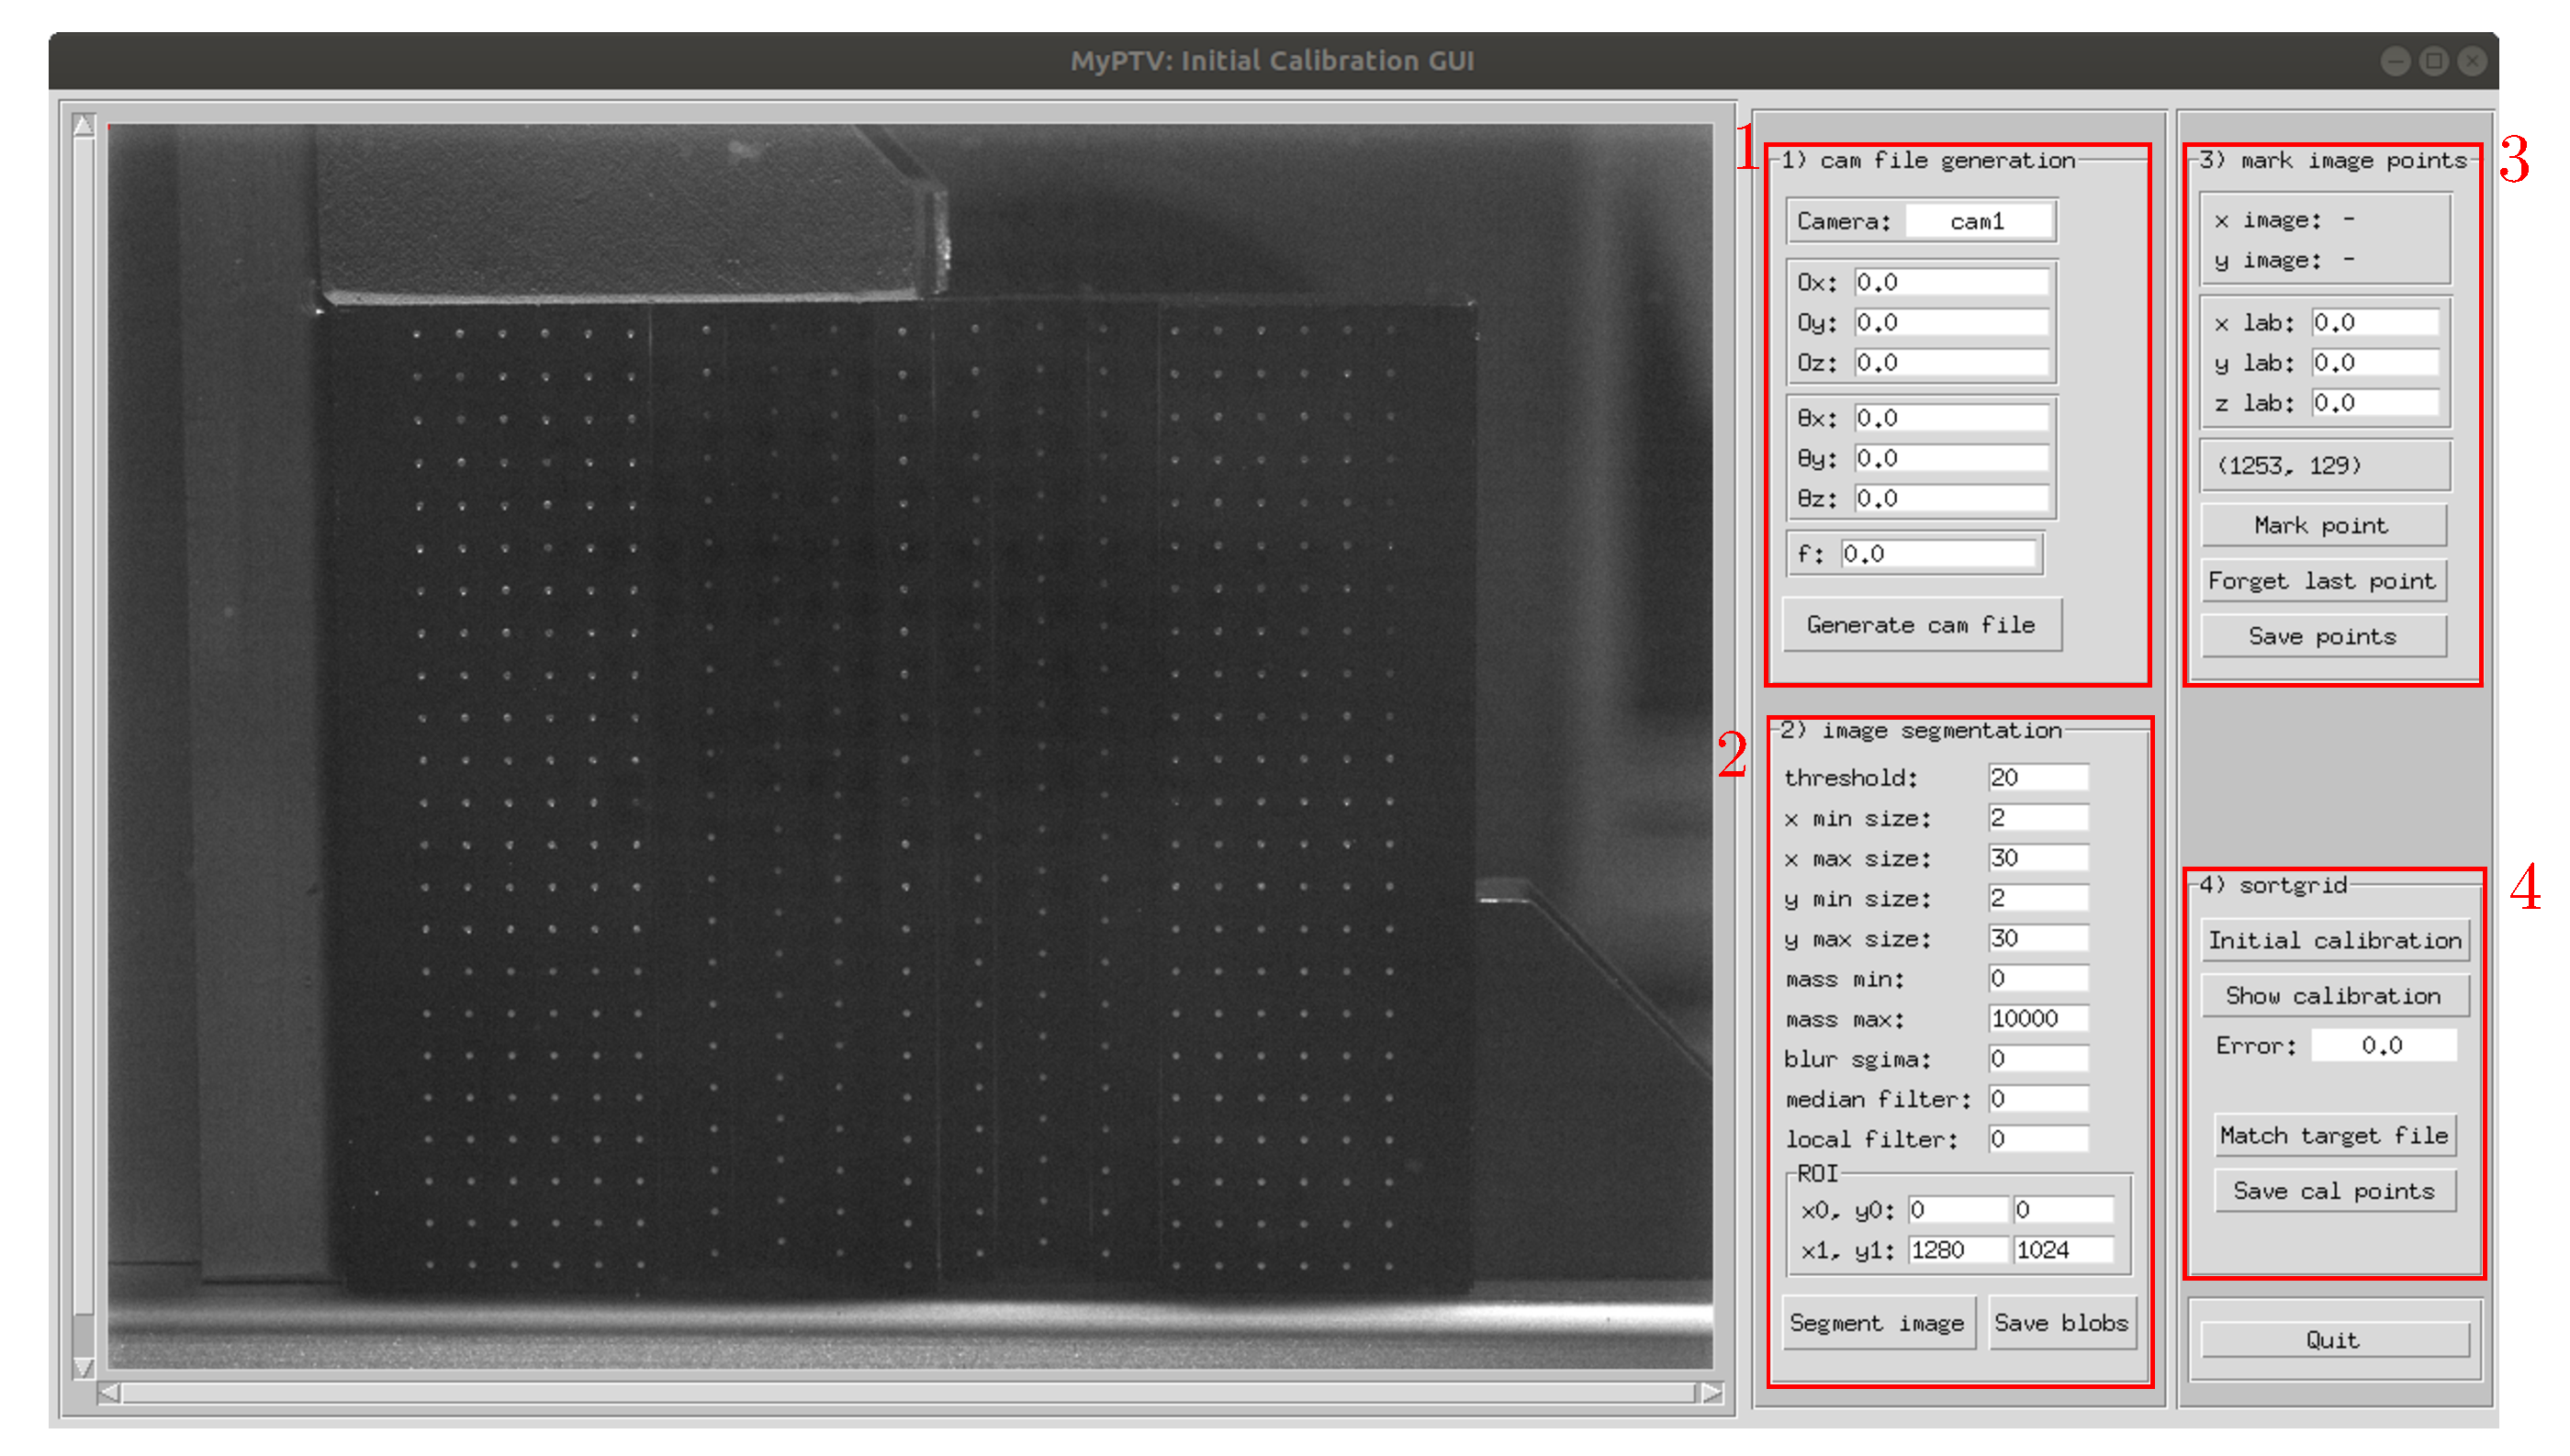
\includegraphics[width=1.0\textwidth]{initial_calibration.pdf}
	\caption{The initial calibration GUI. \label{fig:init_cal_gui}}
\end{figure}


The initial calibration is composed of four steps, and each one has a dedicated panel in the GUI. The steps should, in general, be followed along the order of the steps: 1 $\rightarrow$ 4.   


Here are the details regarding each of the initial calibration steps:

\begin{enumerate}
	\item \texttt{cam file generation}: Here we produce a text file that stores the camera parameters. We first have to give a first guess for the six different external parameters, $\vec{O}$ and $\vec{\theta}$, and the focal length, $f$. It's important to give a reasonably good initial guess, because the calibration problem often has local minima that make the convergence to solution difficult. To understand the how to choose the values, consult Section~\ref{sec:camera_external_params}. When done, click the \texttt{Generate cam file} button.  
	
	\item \texttt{image segmentation}: In this step we use MyPTV to detect the points on the calibration image and to store their pixel coordinates in a file. Choose and tweak the segmentation parameters until all the calibration points are detected (or at least most of them if the images are not ideal). Detected points are indicated by green squares on the image. Also, a reference for the segmentation parameters can be found in Section~\ref{sec:workflow_segment}. Once done, save the file using the \texttt{save} button.
	
	\item \texttt{mark image points}: Here, we start by choosing six points (at least) of the calibration target. The points should not be coplanar and it is best to choose them such that there is some asymmetry to reduce the chance of false convergence. For each point chosen, we mark it by clicking on it on the image and we write its' lab space coordinates in the \texttt{x lab}, \texttt{y lab}, \texttt{z lab} fields, and then click the \texttt{Mark point} button. The marked points will be shown as blue crosses on the image. After marking all the chosen points, we save their coordinates using the \texttt{Save points} button.
	
	\item \texttt{sortgrid}: In this last step, MyPTV tries to calibrate the camera using only the points we marked in step 3, and then to match the calibration points we segmented in step 2 to the points we gave in the target file. Thus, click the \texttt{initial calibration} button, make sure that the calibration error is low (aim for about 1.0), and click \texttt{show calibration}. If the results are good, click the \texttt{Match target file} button, and you should see the segmented points and the associated points from the target file paired by a red line on the image. Make sure that there are no errors in the pairing, and then save the results. If you detect errors or the initial calibration did not reach low enough error, it might be needed to generate an improved initial guess.  
		 
\end{enumerate}
 
This concludes the initial calibration step.

%
%For the initial calibration, follow these steps:
%
%\begin{enumerate}
%	\item \textit{Generate the camera file:} The camera file holds the camera parameters (see Fig.~\ref{fig:camfiles}). An empty camera file can be generated automatically by the workflow script when we start the calibration sequence in a directory that doesn't havea  camera file in it (by running \texttt{python workflow.py params\_file.yml calibration} in the command line).
%	
%	\item \textit{Enter an initial guess:} Open the camera file just generated and insert an initial guess for the camera's position ($\vec{O}$ in the first line), orientation ($\vec{\theta}$ in the second line), and the focal depth ($f$ in the third line). See Section~\ref{sec:camera_external_params} (Understanding camera external parameters) and Fig.~\ref{fig:cam_pos_example} for a reference on how camera translations and orientations and focal lengths are defined. 
%	
%	\item \textit{Segment 6 calibration points:} We start by choosing six points (or more) of the calibration target. The points should not be coplanar and it is best to choose them such that there is some assymetry (e.g. see the blue crosses in Fig.~\ref{fig:Cal_point_GUI}). Then, we need to prepare a file that lets MyPTV know their coordinates in image space and in lab space (see Fig.~\ref{fig:calpointfile} for the format). The name of the file should be inserted under \texttt{calibration\_points\_file} in the \texttt{params\_file.yml}. \\
%	The calibration points file can be generated easily using a dedicated graphical user interface (GUI). To run the GUI, enter \texttt{python workflow.py params\_file calibration\_point\_gui} in the command line. Alternatively, if MyPTV can't find the \texttt{calibration\_points\_file}, the GUI will start automatically. Instruction are given in Fig.~\ref{fig:Cal_point_GUI}.
%	
%	\item \textit{Calibrate using 6 points:} We now calibrate the camera, namely, we optimize the camera parameters such that the calibration error is minimized). This is done using the calibration graphical user interface (GUI), which is initiated by entering \texttt{python workflow.py params\_file.yml calibration} in the command line. The calibration GUI is shown in Fig.~\ref{fig:calibration_gui} and the functionalities are listed in Tab.~\ref{tab:calibration_gui}. In general, we want to observe the calibration error decreasing (the error is the RMS deviation in pixel units). Once the error had converged to a low level, about 1.0 pixels, save the results.
%\end{enumerate}







\begin{figure}
	\centering
	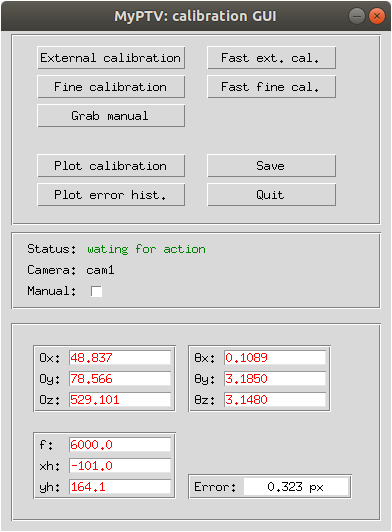
\includegraphics[width=0.4\textwidth]{calibration_gui.png}
	\caption{An image of the calibration GUI. The calibration GUI has several functionalities to run the minimization functions, plot the calibration error and the calibration particle's images, as well as change manually the camera parameters. See Tab.~\ref{tab:calibration_gui} for a description of the operation of each button. \label{fig:calibration_gui}}
\end{figure}



\begin{table}[!ht]
	\centering
	\caption{The various commands available in the calibration GUI (Fig.~\ref{fig:calibration_gui}). \label{tab:calibration_gui}}
	\begin{tabular}{l m{10cm}}
		\hline
		Parameter & Description\\
		\hline
		
		\texttt{External calibration} & Will minimize the calibration error by optimizing the external parameters of the camera using all the calibration points. This might require several runs to reach good results.\\[.3em]
		
		\texttt{Fast ext. cal.} & Will optimize the external camera parameters using a faster stochastic optimizer. This option is good for rapidly obtaining a reasonable calibration when there are a lot of calibration points.\\[.3em]
		
		\texttt{Fine calibration} & Will minimize the calibration error by optimizing the nonlinear error term of the camera parameters. This might require several runs to reach good results. \\[.3em]
		
		\texttt{Fast fine cal.} & Will optimize the nonlinear error terms of the camera parameters using a faster stochastic optimizer. This option is good for rapidly obtaining a reasonable calibration when there are a lot of calibration points.\\[.3em]
		
		\texttt{Grab manual} & This allows to manually change camera parameters. to do this, first tick the \texttt{Manual} checkbox. Then, manually change the values of the camera parameters. Finally, click the button and watch the effect on the calibration error. \\[.3em]
		
		\texttt{Plot calibration} & Will generate a plot of the calibration points projected on the camera space, and the known calibration points.\\[.3em]
		
		\texttt{Plot error hist.} & Will generate a histogram of the calibration errors for the various calibration points. \\[.3em]
		
		\texttt{Save} & Will save the results of the current session in the camera file. \\[.3em]
		
		\texttt{Quit} & Will quit the GUI.\\[.3em]
		\hline
	\end{tabular}
\end{table}





\subsubsection{Understanding camera external parameters} \label{sec:camera_external_params}



The external parameters of a camera in MyPTV include its position, its orientation, and its focal length, $\vec{O}$, $\vec{\theta}$, and $f$, respectively. In the calibration process, it is important to understand these parameters to be able to give a good initial guess and judge the results of the calibration procedure. Thus, let us explain how these parameters are defined.


Each camera is associated with an image space reference frame, shown in Fig.~\ref{fig:cam_pos_example} as the $x',$ $y'$, and $z'$ axes. The $z'$ axis is normal to the imaging plane (the camera's sensor), while $x',$ and $y'$ are tangent to it; the system is right-handed. 


The position parameter, $\vec{O}$, is defined as a vector pointing from the origin of the lab space coordinate system to the origin of the camera's reference frame. It is measured in lab-space units (e.g. millimeters). Therefore, one could estimate $\vec{O}$ directly by using a ruler or a measuring tape to measure where the camera is in the lab-space coordinates. 


The orientation parameter, $\vec{\theta}$, is a vector of three angles that describe the rotation of the camera's reference frame with respect to the lab space frame, namely the camera's Euler angles. The first angle describes the rotation around the $x'$ axis, the second describes rotation around $y'$, and the third angle describes rotation around $z'$. Rules of thumb in trying to guess $\vec{\theta}$ are: 1) ask yourself "how should one rotate the lab's frame of reference so that it aligns with the camera's frame of reference?"; 2) we first rotate around the $x'$ axis, then around $y'$ and then around $z'$. Note: in many cases, the origin of the images is on the top left corner, so half a turn rotation around the $z'$ axis is often needed. See Fig.~\ref{fig:cam_pos_example} for an example.


The focal length parameter,$f$, is essentially an extension factor. In MyPTV $f$ is measured in units of pixels. The focal length is normally more or less equal to the camera's lens focal length. For example, if one uses a camera with a 60mm lens in their experiment, and the size of one camera pixel is 10$\mu$m=0.01mm, then $f$ would roughly be equal to 6000 (pixels). Potentially, one could also estimate $f$ in an experiment: 1) place the camera in a known position facing a calibration target (as e.g. in Fig.4a) and take a picture 2) prepare a calibration points file for a few of the points on the calibration target; 3) preparing a camera file using the known position and orientation 4) insert some initial value for $f$; 5) using the \texttt{workflow.py} file to compare the distribution of the points using this value of $f$; 6) repeat steps 4 and 5 until a fair agreement is found.  

\vspace{.25cm}

\begin{figure}
	\centering
	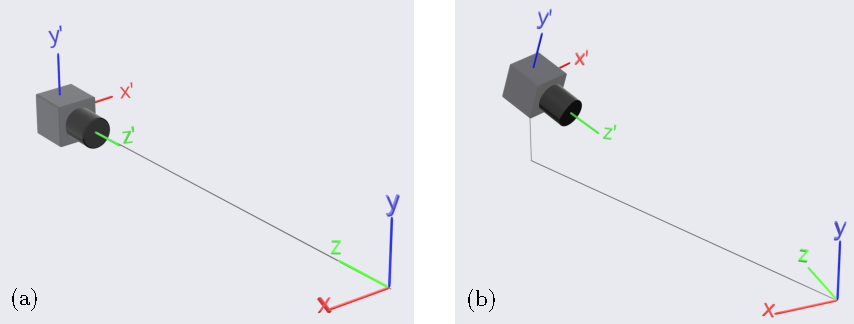
\includegraphics[width=0.8\textwidth]{Cam_pos_examples.pdf}
	\caption{Two examples for camera setups. The (x, y, z) system represents the lab space, and the (x', y', z') represents the camera's system of reference. In (a) the camera's position is roughly $\vec{O} = (0,0,1)$, and an appropriate rotation vector could be $\vec{\theta} = (0,\pi,0)$. In (b) the camera's position might be $\vec{O} = (1,1,1)$, and the orientation vector might approximately be $\vec{\theta} = (-\frac{1}{2}\pi,-\frac{3}{4}\pi,0)$. \label{fig:cam_pos_example}}
\end{figure}



%\vspace{.5cm}
%
%\begin{figure}[!ht]
%\begin{center}
%	
%	\fcolorbox{white}{bcolor}{
%	\begin{minipage}[c][][c]{0.95\textwidth}
%		
%		\vspace{.1cm}
%		
%		\textbf{Understanding camera external parameters:} The external parameters of a camera in MyPTV include its position, its orientation, and its focal length, $\vec{O}$, $\vec{\theta}$, and $f$, respectively. In the calibration process, it is important to understand these parameters to be able to give a good initial guess and judge the results of the calibration procedure. Thus, let us explain how these parameters are defined.
%		
%		\vspace{.5cm}
%		
%		Each camera is associated with an image space reference frame, shown in Fig.~\ref{fig:cam_pos_example} as the $x',$ $y'$, and $z'$ axes. The $z'$ axis is normal to the imaging plane (the camera's sensor), while $x',$ and $y'$ are tangent to it; the system is right-handed. 
%		
%		\vspace{.25cm}
%		
%		The position parameter, $\vec{O}$, is defined as a vector pointing from the origin of the lab space coordinate system to the origin of the camera's reference frame. It is measured in lab-space units (e.g. millimeters). Therefore, one could estimate $\vec{O}$ directly by using a ruler or a measuring tape to measure where the camera is in the lab-space coordinates. 
%		
%		\vspace{.25cm}
%		
%		The orientation parameter, $\vec{\theta}$, is a vector of three angles that describe the rotation of the camera's reference frame with respect to the lab space frame, namely the camera's Euler angles. The first angle describes the rotation around the $x'$ axis, the second describes rotation around $y'$, and the third angle describes rotation around $z'$. Rules of thumb in trying to guess $\vec{\theta}$ are: 1) ask yourself "how should one rotate the lab's frame of reference so that it aligns with the camera's frame of reference?"; 2) we first rotate around the $x'$ axis, then around $y'$ and then around $z'$. Note: in many cases, the origin of the images is on the top left corner, so half a turn rotation around the $z'$ axis is often needed. See Fig.~\ref{fig:cam_pos_example} for an example.
%		
%		\vspace{.25cm}
%		
%		The focal length parameter,$f$, is essentially an extension factor. In MyPTV $f$ is measured in units of pixels. The focal length is normally more or less equal to the camera's lens focal length. For example, if one uses a camera with a 60mm lens in their experiment, and the size of one camera pixel is 10$\mu$m=0.01mm, then $f$ would roughly be equal to 6000 (pixels). Potentially, one could also estimate $f$ in an experiment: 1) place the camera in a known position facing a calibration target (as e.g. in Fig.4a) and take a picture 2) prepare a calibration points file for a few of the points on the calibration target; 3) preparing a camera file using the known position and orientation 4) insert some initial value for $f$; 5) using the \texttt{workflow.py} file to compare the distribution of the points using this value of $f$; 6) repeat steps 4 and 5 until a fair agreement is found.  
%		
%		\vspace{.25cm}
%		
%		\begin{center}
%			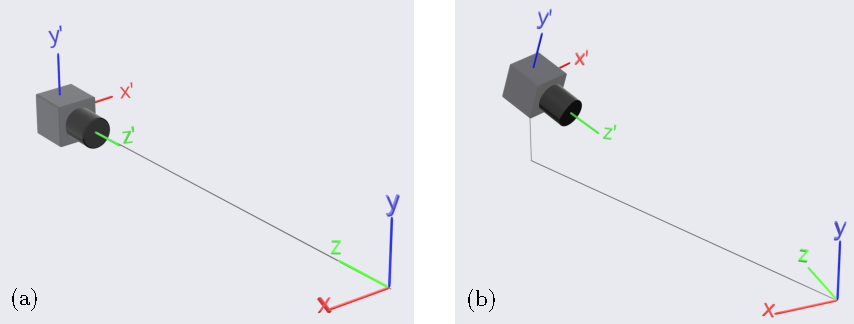
\includegraphics[width=\textwidth]{Cam_pos_examples.pdf}
%			\caption{Two examples for camera setups. The (x, y, z) system represents the lab space, and the (x', y', z') represents the camera's system of reference. In (a) the camera's position is roughly $\vec{O} = (0,0,1)$, and an appropriate rotation vector could be $\vec{\theta} = (0,\pi,0)$. In (b) the camera's position might be $\vec{O} = (1,1,1)$, and the orientation vector might approximately be $\vec{\theta} = (-\frac{1}{2}\pi,-\frac{3}{4}\pi,0)$. \label{fig:cam_pos_example}}
%		\end{center}
%		
%		
%		\vspace{.1cm}
%		
%	\end{minipage}
%	}
%\end{center}
%
%\end{figure}



%\begin{figure}[!ht]
%	\centering
%	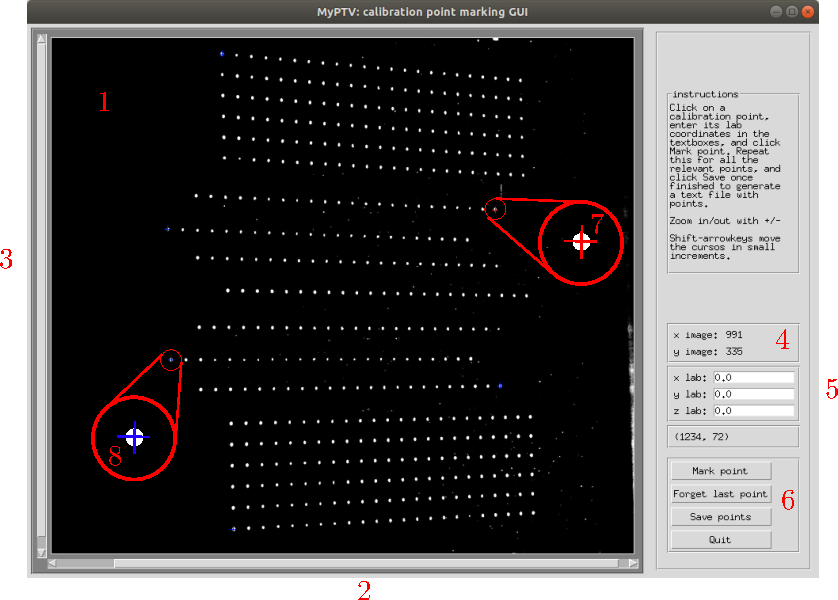
\includegraphics[width=0.85\textwidth]{Cal_point_GUI.pdf}
%	\caption{The calibration point segmentation GUI. 1 - the calibration image, with points to be segmented. 2 and 3 - scroll bars to explore the image. When the image is clicked a red cross apears (7) and its coordinates in image space are pronted in 4; to mark a calibration point click on it. 5 - to specify the lab space coordinates of the point, enter them in the correct tabs. 6 - once 'mark point' is clicked, the cross becomes blue (8), which means that the point's data was registered in the memory. to remove points from the register click 'Forget last point'. To save the points in the register click 'Save points' (the file name is the one given in \texttt{calibration\_points\_file}). To zoom in use the +/- buttons. To move the red cross more accurately, use Shift-Arrowkey. \label{fig:Cal_point_GUI}}
%\end{figure}


\begin{figure}[!ht]
	\centering
	%
	\subfloat[]{ \label{fig:calpointfile}
		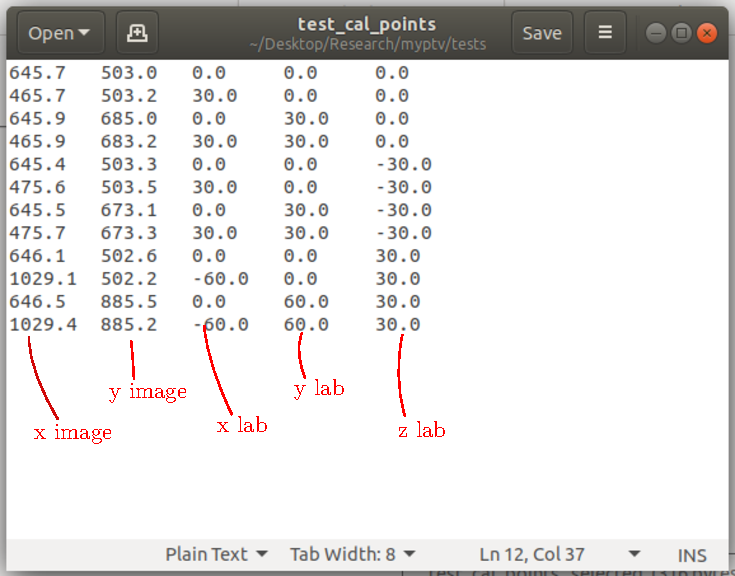
\includegraphics[width=7cm]{cal_point_file.pdf}
	}\\
	%
	\subfloat[]{\label{fig:target_file}
		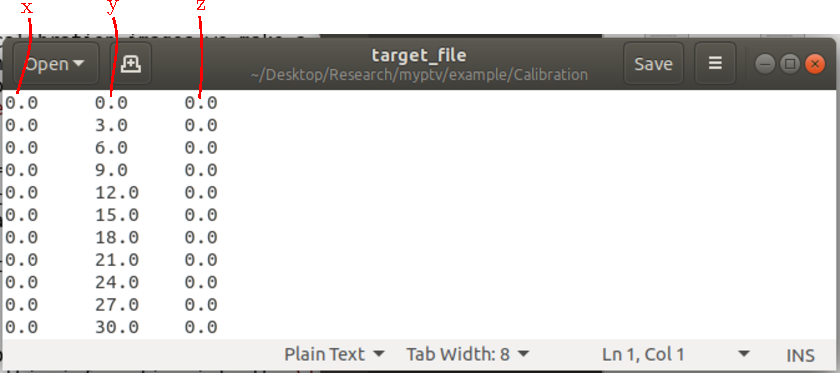
\includegraphics[width=9cm]{target_file.pdf}}
	%
	\subfloat[]{\label{fig:match_target_file}
		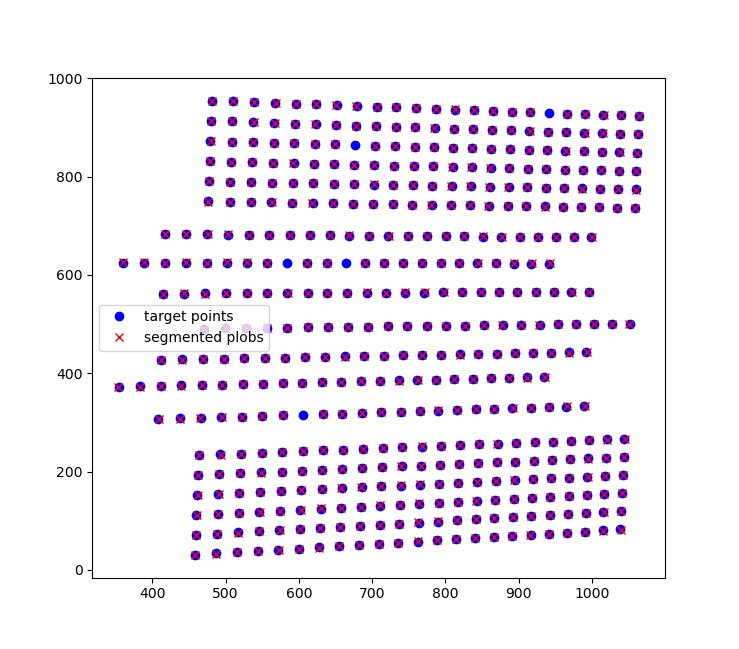
\includegraphics[width=6.0cm]{match_target_file.jpeg}}
	%
	\caption{(a) Format of the target file, which lists the lab-space coordinates of the calibration target as tab-separated values. The order at which points are given is not relevant. (b) An example of a text file holding the calibration point data. (c) The results of matching a target file points (blue circles) and the segmented blobs (red crosses). Here, we know that the match is correct because each cross overlays a circle. In location where circles are not overlaid by a cross, the segmentation did not recognize a calibration target; having such missing points may slightly reduce the quality of the calibration but it is not critical for the target file matching.}
\end{figure}



\subsubsection{Final calibration}

In the final calibration we use all the calibration points to find the parameters of the camera. We do this by minimizing the calibration error, defined as the root mean square of the distances between the image-space calibration points positions and the projection of the lab-space points on the image plane. The minimization is solved numerically using the \textit{final calibration gui}. 


To start the final calibration gui, use the workflow script with the following command:
%
\begin{verbatim}
python workflow.py params_file.yml final_calibration
\end{verbatim}
%
which should start the interface shown in Fig.~\ref{fig:calibration_gui}. The description of each of the possible functionalities are given in Table~\ref{tab:calibration_gui}. In principal, the lower the calibration error, the results of the measurements will be more reliable, and it will become possible to track a higher number of particles in each frame. A good calibration will have an error lower than about 0.5, or even 0.3 pixels. Once a good error value is achieved, the calibration process is complete. 



%
%
%For the final calibration, follow these steps:
%
%
%\begin{enumerate}
%	\item \textit{Prepare a target file:} If there is no target file in the experimental folder, this is the time to generate one. A \textit{target file} is a text file which lists the lab-space coordinates of all the points on our calibration target according to the format shown in Fig.~\ref{fig:target_file}. Prepare such a file and save it in the experiment's calibration folder.
%	
%	\item \textit{Segment the calibration points:} To obtain the image space coordinates of all the calibration points we use the segmentation operation of the workflow script. To do so: 1) insert the name of the calibration image under the \texttt{Segmentation -> single\_image\_name} tab; 2) run the segmentation command - \texttt{python workflow.py params\_file.yml segmentation}. If the results are not satisfactory, change the segmentation parameters and re-run the segmentation command until you get it; then save the results (the file name used is the one under the \texttt{segmented\_points\_file} field in the \texttt{params\_file}). See also Sec.~\ref{sec:workflow_segment} for more details on the segmentation process.  
%	
%	\item \textit{Match points to target file:} Here we let MyPTV know which of the segmented points corresponds to which point in the target file. To do this, we used the command \texttt{python workflow.py params\_file.yml match\_target\_file}. This will generate a figure, highlighting the target file and the segmented results  by one another. Make sure that the two data match each other (see Fig.~\ref{fig:match_target_file}. If the results are good, save them by quitting the figure and entering 1 when prompted. If the match is not good, then the initial calibration was not good enough; enter 2 when prompted, and return to Sec.~\ref{sec:init_calibration} to improve the initial calibration.
%	
%	\item \textit{Calibrate using all points:} Now that we have segmented the necessary data, we return to the calibration GUI by running \texttt{python workflow.py params\_file.yml calibration} in the command line. Use the GUI to reduce the calibration error as much as possible. Values lower that 0.5 pixels or even 0.3 should be sought.  
%\end{enumerate}














%
%\subsubsection{Segmenting the calibration images and matching the target file}
%
%
%To prepare for the final calibration, we need to prepare a \textit{calibration points file} for the rest of the calibration points on our target. To avoid inserting the information for each point manually, we use a semi-automated process as follows:
%%
%\begin{enumerate}
%	\item Segment the calibration target points in the calibration image using the workflow script, as outlined in Sec.~\ref{sec:workflow_segment}. Save the segmented calibration points in the experiment's Calibration folder with a name such as \texttt{blobs\_cam1}. Insert the name of this file under the \texttt{segmented\_points\_file} field of the \texttt{params\_file.yml} file.
%	
%	\item Open the command line on the experiment directory, and run the workflow script with the following command:
%	\begin{verbatim}
%	python workflow.py params_file.yml match_target_file
%	\end{verbatim}
%	
%	\item After automated sorting, a figure window should appear. Make sure that the blue points are overlaid with the red X's and close the figure window. Follow the instructions to save the calibration points file (under the name given in the \texttt{params\_file.yml} under\\ \texttt{calibration\_points\_file}). 
%\end{enumerate}
%
%You should now have a file that contains the full information of the calibration points. Proceed with the fine calibration process.
%
%
%
%
%
%
%\subsubsection{Calibration workflow}\label{sec:cam_cal}
%
%
%Once all the data files are ready in the experiment folder, we use the workflow script to minimize the calibration error by tuning the cameras' external parameters and correction terms. Thus:
%
%\begin{enumerate}
%	
%	\item Start a terminal (or command line prompt), and change directory to the experiment's folder:
%	\begin{verbatim}
%	cd \path\to\the\experiment\folder
%	\end{verbatim}
%	
%	\item Enter the following command:
%	\begin{verbatim}
%	python workflow.py params_file.yml calibration
%	\end{verbatim}
%	
%	\item If a camera file does not yet exist in the folder, MyPTV had just generated an empty one for you. Locate this file in the experiment folder, enter an initial guess for the external parameters and save the file.
%	
%	\item If a camera file exists in the exprimental folder, an interactive dialogue should now appear in the terminal which offers:
%	\begin{verbatim}
%	1 - external parameters minimization 
%	2 - correction error term calibration
%	3 - print current camera parameters
%	4 - plot the projection of the calibration points
%	8 - save the current calibration results
%	9 - quit
%	\end{verbatim}
%	Thus, proceed using options 1 and 2 in iterations and note the calibration error decreasing. Once satisfied, save the results.
%	
%\end{enumerate}
%	


\subsubsection{Important notes}

\begin{enumerate}
	\item A "good" calibration will have a low error value - less than 0.5 pixels.  
	
	\item Optional validation - After all the cameras have been calibrated, it is also good practice to verify the calibration solution by stereo matching the calibration points. To do this, we use the \texttt{match\_blob\_files} (Section~\ref{sec:matching}) to stereo match the files of the segmented calibration target points. We can then calculate the so-called \textit{static calibration error} by computing the RMS of the distance between the triangulated calibration points and the real data from the target file. See Fig.~\ref{fig:cal_err} for an example. This validation step is not yet implemented in the workflow script. 
\end{enumerate}




\begin{figure}[h!]
	\centering
	%
	\subfloat[]{\label{fig:cal_img}
		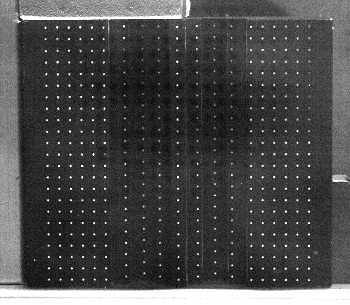
\includegraphics[height=6cm]{cal_image.jpg}}
	\hfill
	%
	\subfloat[]{\label{fig:cal_err}
		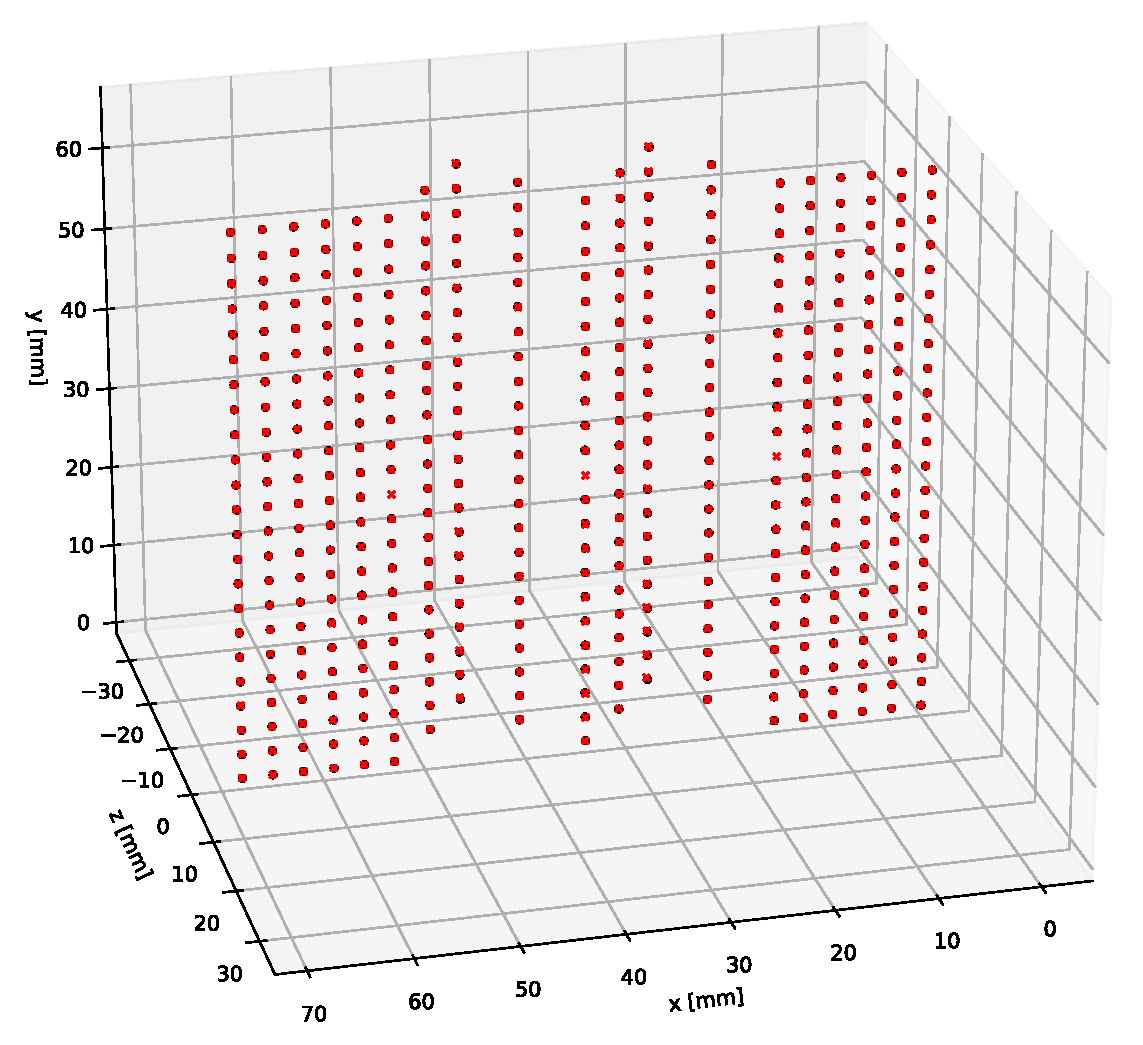
\includegraphics[height=6cm]{cal_error.pdf}}
	%
	\caption{(a) An example of a calibration image. The points on the target have known lab space coordinates. Not also that the points are distributed over several plains (3 different $z$ values in this case). (b) An example plot of a calibration error estimation. The red crosses represent the known positions of the calibration points given in the target file, and the black circles mark the positions of the stereo-matched segmented calibration points. In this case, the root mean square of the static calibration error was 84$\mu m$.}
\end{figure}




\subsection{Segmentation}\label{sec:workflow_segment}




\subsubsection{How segmentation works} In the segmentation step, the program extracts the location of particles in the image. Segmentation in MyPTV is performed in one of two methods: \textit{labeling}, or \textit{dilation}, and includes several optional image processing steps. 


\begin{enumerate}
	\item In the labeling method, we first choose all pixels in an image whose grey value is higher than a given threshold. Then, such pixels that are touching each other are considered to be "blobs", so we group them together. For each blob, we calculate a \textit{center of mass}, being the grey value weighted average of the blob, a \textit{bounding box} size, and a \textit{mass}, being the sum of grey values of the blobs' pixels.
	
	\item In the dilation method, we are looking for pixels that their grey value is higher than that of all their neghbours within a box of a given size (\texttt{particle\_size}), and thet their grey value is higher than a given threshold. After that, all the neighbouring pixels inside the particle size box are considered to be a blob. We then calculate the center of mass of the blob to achieve a better estimation of its position, thus redifining the blob. This process is iterated a maxinum of 3 times untill convergence is obtained. Finally, we calculate the same blob's \textit{center of mass}, \textit{bounding box} size, \textit{mass}.
\end{enumerate}



To improve the results of segmenting over non-ideal images, MyPTV can be set to apply image processing before the blob extraction. The filters that can be used are a Gaussian blur filter, a median noise removal filter, local mean subtraction filter, and a mask. The first three filters may increase the computational time, however they may be necessary depending on the experimental conditions, such as uneven illumination or noisy images. Examples of the results of using several combinations of the filters on a calibration image is shown in Fig.~\ref{fig:image_filters}. 


\begin{figure}[h!]
	\centering
	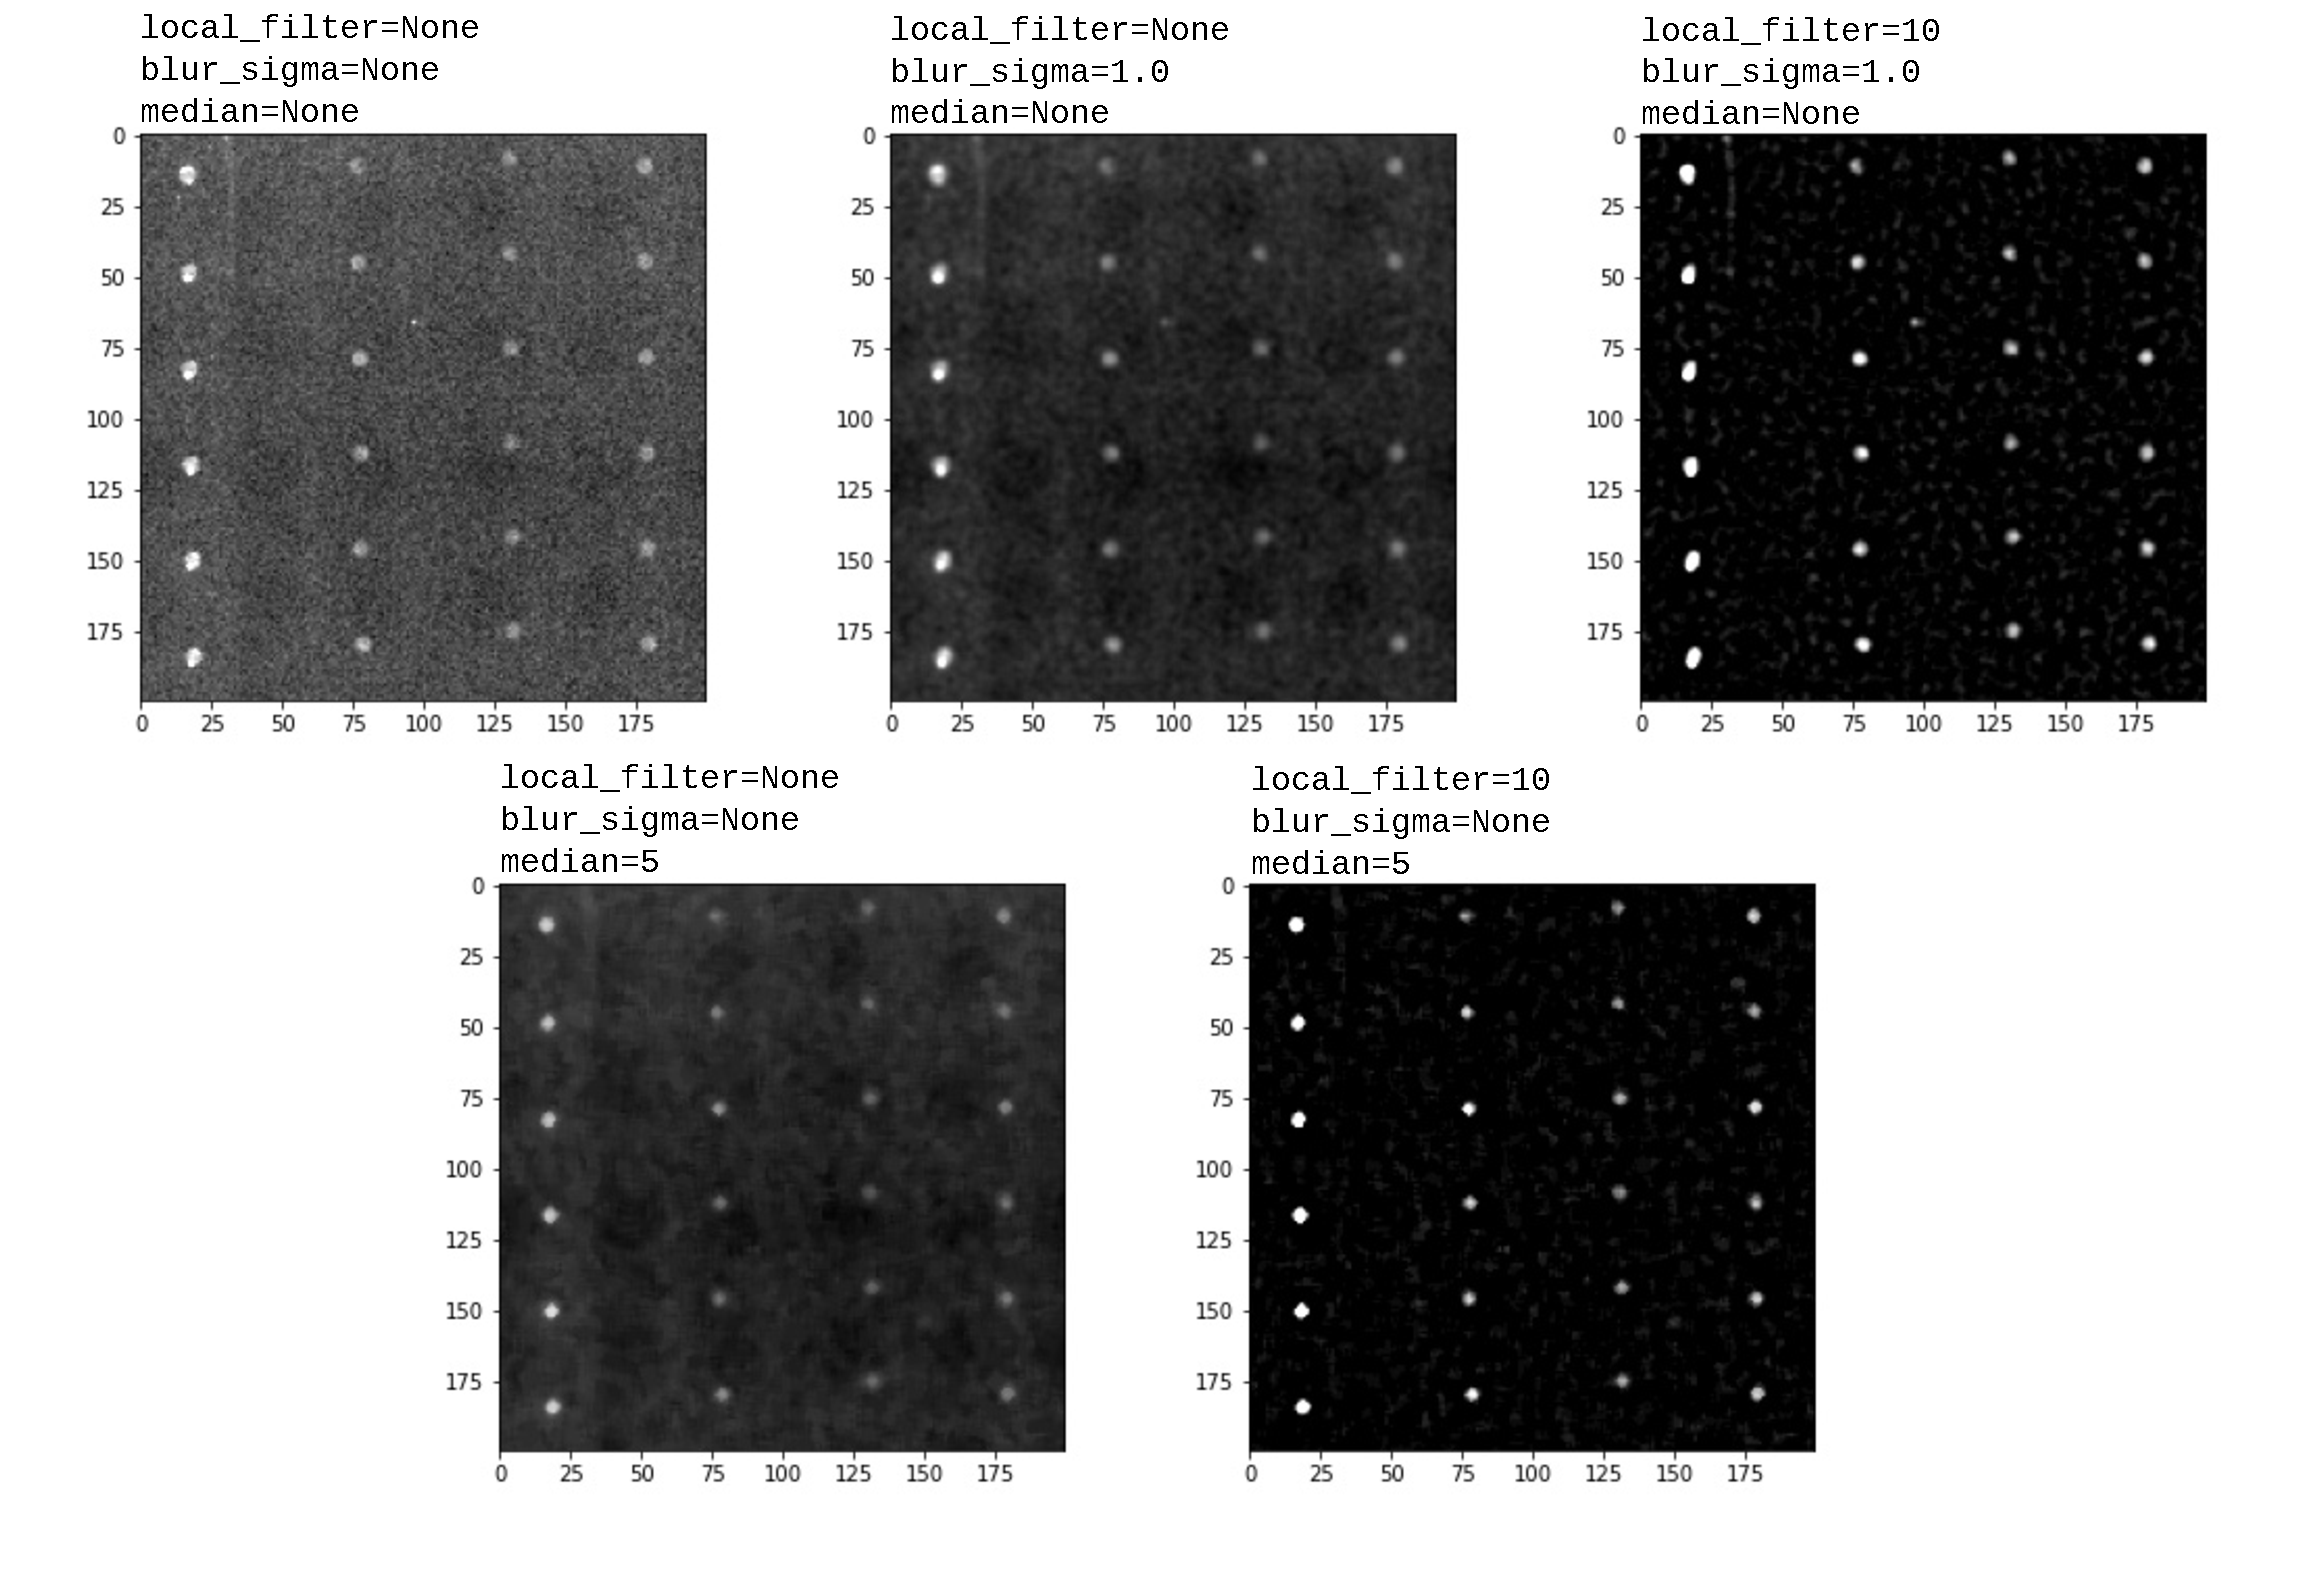
\includegraphics[width=12cm]{filters_effect.pdf}
	\caption{The effect oft various image filters on the segmentation.\label{fig:image_filters}}
\end{figure}




In this step we extract the particles' image-space coordinates from the images and save the coordinates in dedicated files. Use the \texttt{workflow.py} script with the \texttt{segmentation} command to start the process:

\begin{enumerate}
	\item We perform the segmentation first on a single image by specifying \texttt{Number\_of\_images: 1}, and giving an image name with \texttt{single\_image\_name}. We then tune the segmentation parameters and the image processing filters used (e.g. \texttt{ROI}, \texttt{threshold}, \texttt{blur\_sigma}, \texttt{method} etc; the full list is given in Table~\ref{tab:segment_params}) to obtain optimal results; optionally repeat over several more images to ensure the results are satisfactory. To view the segmented particles over the image, use \texttt{plot\_result: True}, and make sure the results are not saved by using \texttt{save\_name: None}. 
	
	\item Once the parameters are determined, we set \texttt{Number\_of\_images: None}, and run the segmentation workflow again. This will then loop over all the images in the given folder (under \texttt{images\_folder}), and save the results in a text file by setting \texttt{save\_name: /file/name/to/use}
\end{enumerate}








\begin{table}[!ht]
	\centering
	\caption{The \texttt{params\_file.yml} parameters for the segmentation step. All paths to files are relative to the \texttt{workflow.py} script. \label{tab:segment_params}}
	\begin{tabular}{l m{10cm}}
		\hline
		Parameter & Description\\
		\hline
		
		\texttt{image\char`_start} & The number of the image from which the loof begins. If this is \texttt{None} (default) the first image is set to 0.\\[.3em]
		
		\texttt{Number\char`_of\char`_images} & Number of images over which to do the segmentation. If it is 1, segmentation is done only on the image with the name given in \texttt{single\char`_image\char`_name}. If this is an integer, segmentation is performed on the first N images found in the directory \texttt{images\char`_folder}. If this is \texttt{None}, segmentation is performed over all the images in the directory \texttt{images\char`_folder} \\[.3em]
		
		\texttt{images\char`_folder} & path to the folder containing the images\\[.3em]
		
		\texttt{single\char`_image\char`_name} & If \texttt{Number\char`_of\char`_images} is 1, the segmentation will be done on the image whose name is given here. If \texttt{Number\char`_of\char`_images} is any other value, this parameter is not used. \\[.3em]
		
		\texttt{image\char`_extension} & extension of the images; for example, .tif\\[.3em]
		

		\texttt{plot\_result} & if \texttt{False} will not plot the results; if \texttt{True} the results will be plotted but only if number of images is 1 \\[.3em]
		
		\texttt{mask} & if this is 1.0, no mask is used; if this is set to a path to a file, the file will be used as a mask for the segmentation \\[.3em]

		
		\texttt{ROI} & region of interest; specify by indicating the xmin, xmax, ymin, ymax coordinates \\[.3em]
		
		\texttt{threshold} & the brightness value for which a point is considered a particle after a local mean subtraction is performed \\[.3em]
		
		\texttt{median} & the intger window size of a median noise removal filter; set to \texttt{None} in order to not apply the filter \\[.3em]
		
		\texttt{blur\_sigma} & the float standard deviation of a Gaussian blur filter; set to \texttt{None} in order to not apply the filter \\[.3em]
		 
		\texttt{local\_filter} & the integer widow size of a local mean subtraction filter; set to \texttt{None} in order to not apply the filter \\[.3em]
		
		\texttt{min\_xsize} & minimum particle size (pixels) in $x$ direction \\[.3em]
		
		\texttt{min\_ysize} & minimum particle size (pixels) in $y$ direction \\[.3em]
		
		\texttt{min\_mass} & minimum particle mass (mass is the sum of pixel grey values)\\[.3em]
		
		\texttt{max\_xsize} & maximum particle size (pixels) in $x$ direction \\[.3em]
		
		\texttt{max\_ysize} & maximum particle size (pixels) in $y$ direction \\[.3em]
		
		\texttt{max\_mass} & maximum particle area (mass is the sum of pixel grey values) \\[.3em]

		\texttt{plot\_result} & if \texttt{True} the segmented particles will be plotted over the processed image (after applying blur, local mean subtraction and masking); if \texttt{False} will not plot the results \\[.3em]
		
		\texttt{method} & ihe name of the method used for segmenting the blobs; can be either 'labeling' or 'dilation' \\
		
		\texttt{particle\_size} & in the 'dilation' method, this gives the diameter of blobs in the image (an integer number of pixels); this parameter is not used when method is set to 'labeling' \\
		
		\texttt{save\_name} & if \texttt{None} the results will not be saved in a file; if \texttt{path/to/file} will save the results in the given file name \\
		
		\hline
	\end{tabular}
\end{table}








\subsection{Matching}\label{sec:workflow_match}

In the matching step, particles images in the various images are used to stereo-locate (triangulate) the 3D positions of particles in the lab-space coordinates. As before, run first only on several images to find optimal parameter values, and only then iterate over all frames by setting \texttt{N\_frames: None} and save the results. 


\begin{table}[!ht]
	\centering
	\caption{The \texttt{params\_file.yml} parameters for the matching step. All paths to files are relative to the \texttt{workflow.py} script.}
	\begin{tabular}{l m{10cm}}
		\hline
		Parameter & Description\\
		\hline
		
		\texttt{blob\_files} & names of files that hold the segmented particles for each camera, separated by commas; for example: \texttt{blobs\_cam1, blobs\_cam2, blobs\_cam3} \\
		
		\texttt{frame\_start} & if \texttt{None} will start matching from the first available frame. If an integer it will start the matching from this given number. \\
		
		\texttt{N\_frames} & if \texttt{None} will match particles in all available frames; if an integer will match only particles in the first \texttt{N} frames. \\
		
		\texttt{camera\_names} & names of cameras used separated by commas; for example, \texttt{cam1, cam2, cam3} \\
		
		\texttt{cam\_resolution} & camera resolution; for example, \texttt{1280, 1024} \\
		
		\texttt{ROI} & region of interest for the matching in lab space coordinates, and according to the format of \texttt{xmin, xmax, ymin, ymax, zmin, zmax} \\
		
		\texttt{voxel\_size} & the side length of voxels used in the \textit{Ray Traversal} algorithm; note - too high values lead to long computation times and too low value result in matching errors and long computation times. \\
		
		\texttt{max\_blob\_distance} &  the distance particle usually undergo during each frame in image space coordinates (pixels)\\
		
		\texttt{max\_err} & maximum value of the RMS triangulation error in lab space coordinates \\
		
		\texttt{save\_name} & path name used for saving the results; if \texttt{None} the results are not saved \\
		
		\hline
	\end{tabular}
\end{table}




%\vspace{.5cm}
%
%\begin{center}	
%	\fcolorbox{white}{bcolor}{
%		\begin{minipage}[c][][c]{1.0\textwidth}
%			
%			\vspace{.1cm}
%			
%			\textbf{How segmentation works:} Segmentation in MyPTV is performed in one of two methods: \textit{labeling}, or \textit{dilation}, and includes several optional image processing steps. 
%			
%			\vspace{.2cm}
%			
%			\begin{enumerate}
%				\item In the labeling method, we first choose all pixels in an image whose grey value is higher than a given threshold. Then, such pixels that are touching each other are considered to be "blobs", so we group them together. For each blob, we calculate a \textit{center of mass}, being the grey value weighted average of the blob, a \textit{bounding box} size, and a \textit{mass}, being the sum of grey values of the blobs' pixels.
%				
%				\item In the dilation method, we are looking for pixels that their grey value is higher than that of all their neghbours within a box of a given size (\texttt{particle\_size}), and thet their grey value is higher than a given threshold. After that, all the neighbouring pixels inside the particle size box are considered to be a blob. We then calculate the center of mass of the blob to achieve a better estimation of its position, thus redifining the blob. This process is iterated a maxinum of 3 times untill convergence is obtained. Finally, we calculate the same blob's \textit{center of mass}, \textit{bounding box} size, \textit{mass}.
%			\end{enumerate}
%			
%			\vspace{.2cm}
%			
%			To imrove the results of segmenting over non-ideal images, MyPTV can be set to apply image processing before the blob extraction. The fiters that can be used are a gaussian blur filter, a median noise removal filter, local mean subtraction filter, and a mask. The first three filters may increase the computational time, however they may be necessary depending on the experimental conditions, such as uneven illumination or noisy images. Examples of the results of using several combinations of the filters on a calibration image is shown below. 
%			
%			\vspace{.2cm}
%			
%			\begin{center}
%				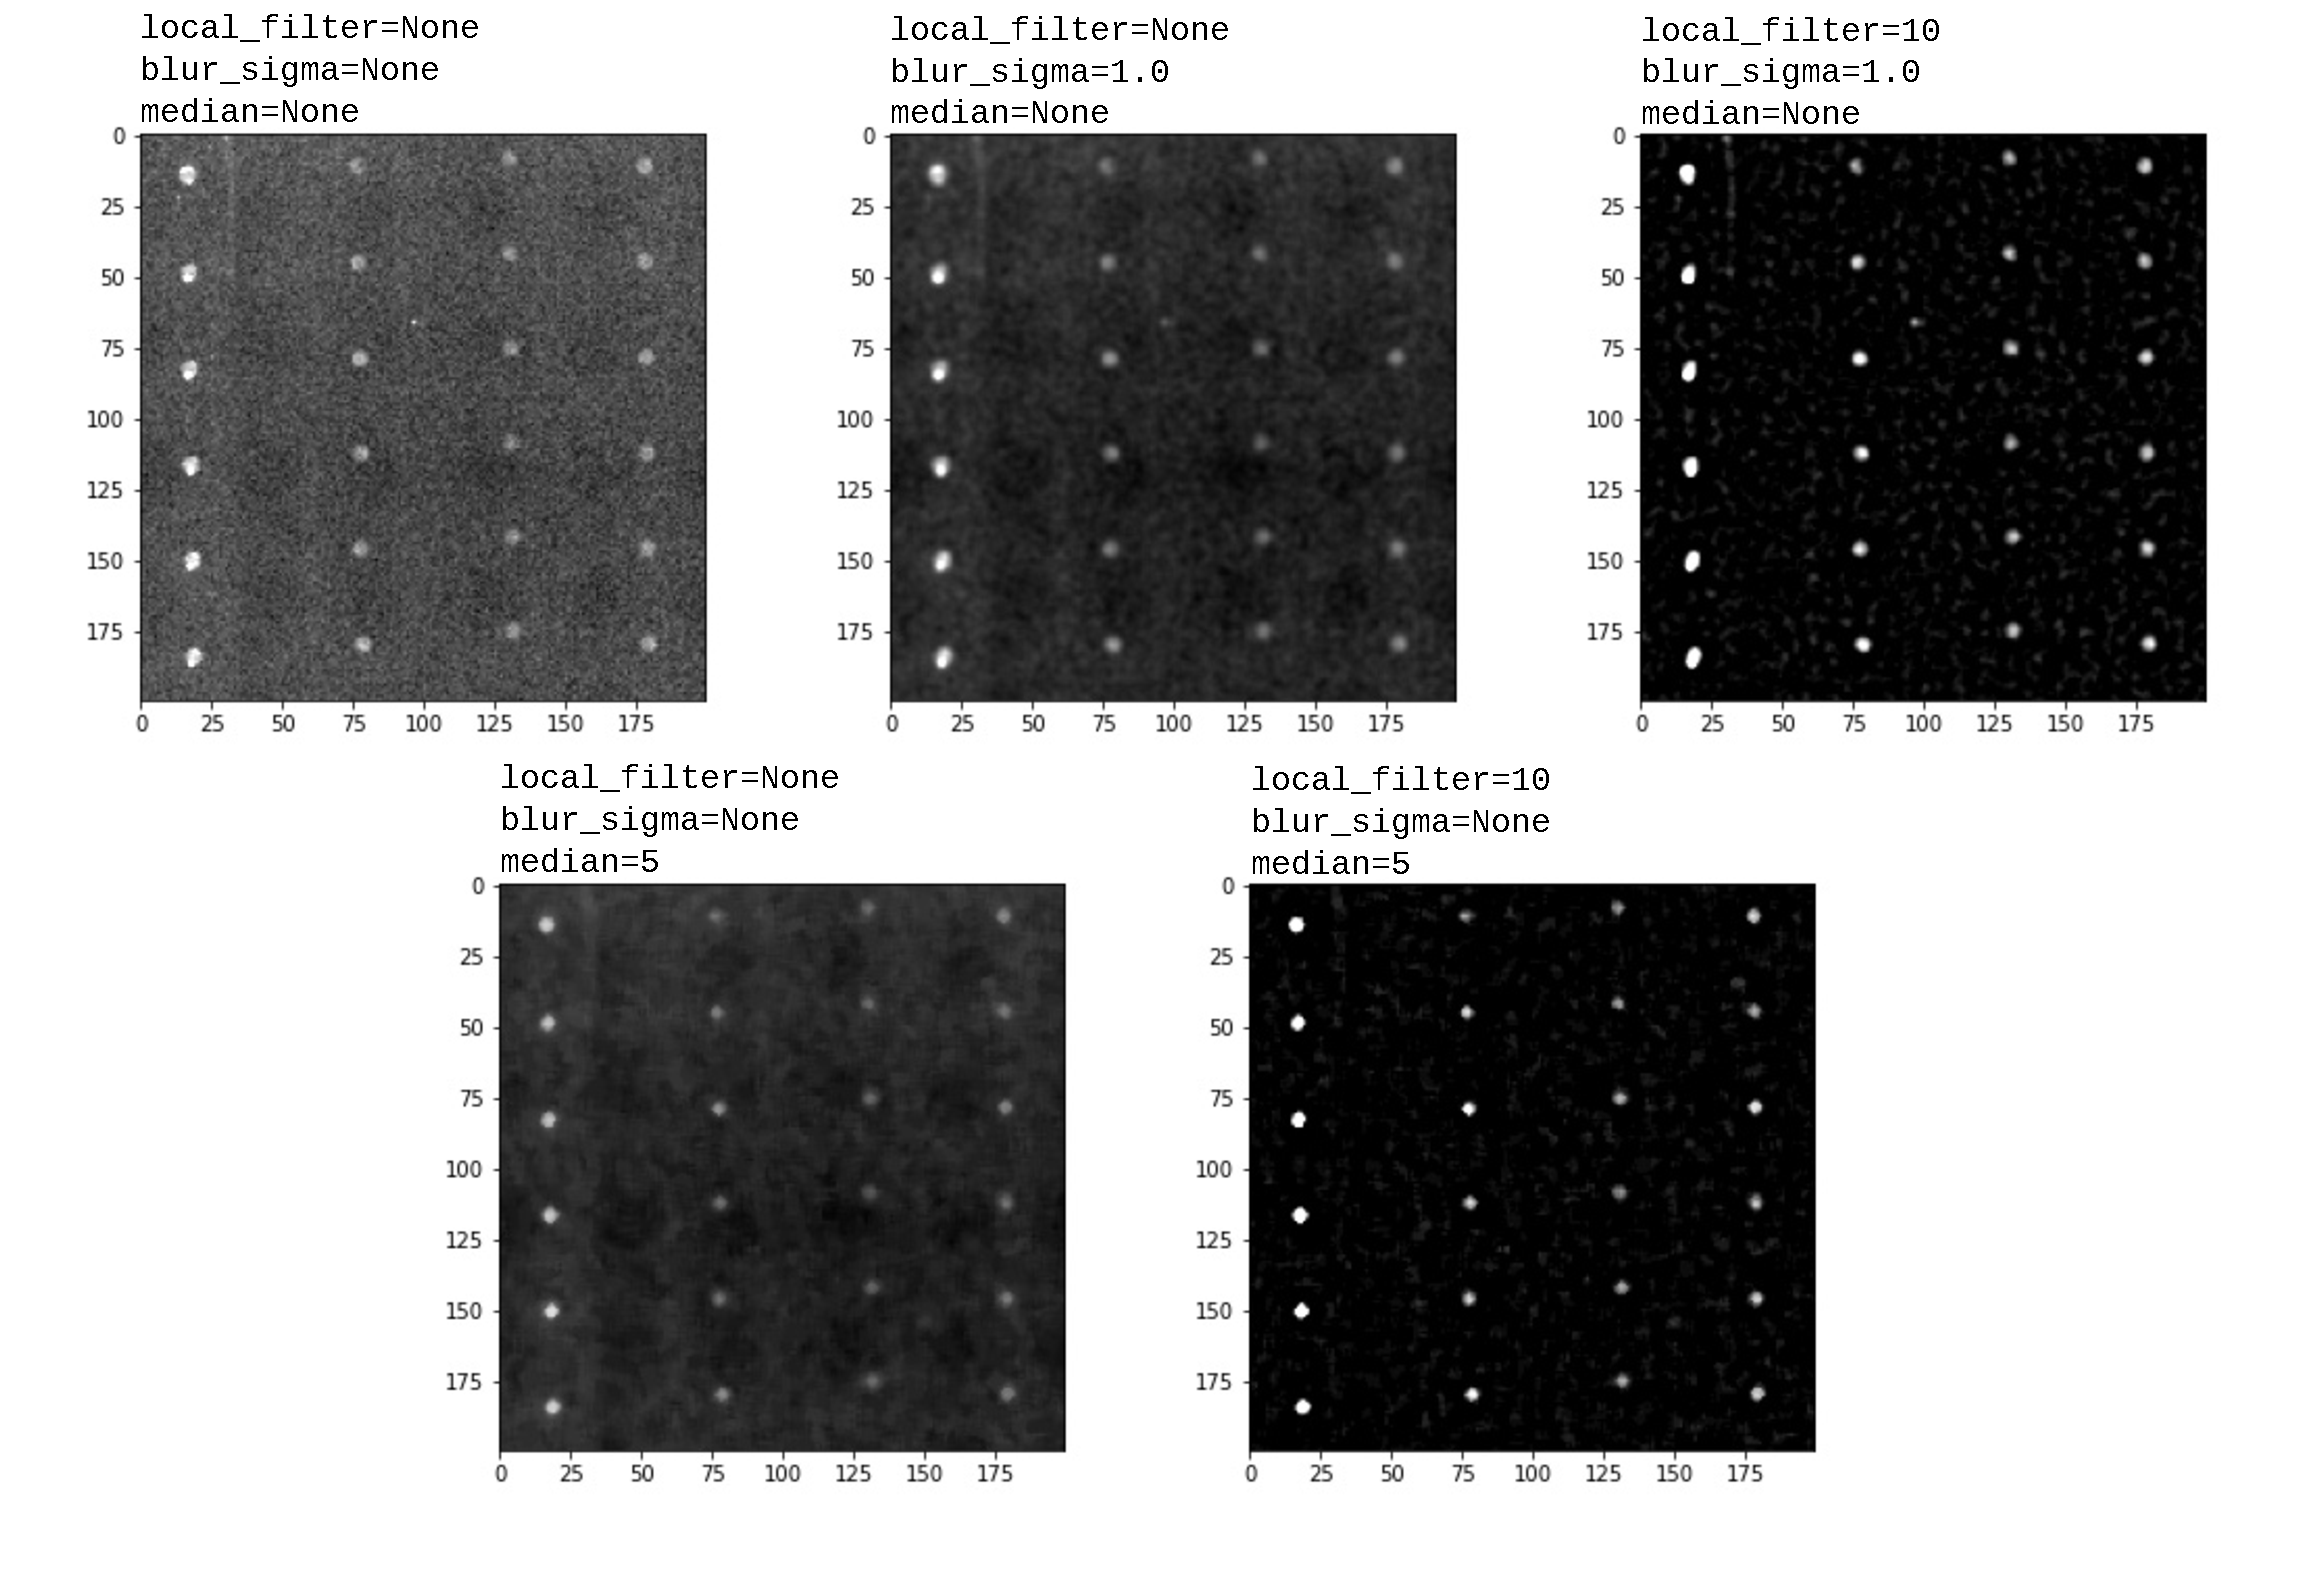
\includegraphics[width=7cm]{filters_effect.pdf}
%			\end{center}
%			
%			\vspace{.1cm}
%			
%		\end{minipage}
%	}
%	
%\end{center}



\subsection{Tracking}\label{sec:workflow_track}

The tracking step is used to link particle in the lab space coordinates in time, thus forming the 3D trajectories.




\begin{table}[!ht]
	\centering
	\caption{The \texttt{params\_file.yml} parameters for the tracking step. All paths to files are relative to the \texttt{workflow.py} script.}
	\begin{tabular}{l m{10cm}}
		\hline
		Parameter & Description\\
		\hline
		
		\texttt{particles\_file\_name} & path name of the file which holds the 3D coordinates of particles, namely the results of the matching step  \\
		
		\texttt{frame\_start} & if \texttt{None} will start tracking from the first available frame. If an integer it will start the tracking from this given number. \\
		
		\texttt{N\_frames} & if \texttt{None} will iterate over particles in all frames; if an integer will only track particles in the first \texttt{N} frames of the particles file\\
		
		\texttt{d\_max} & the maximum translation in lab space coordinates \\
		
		\texttt{dv\_max} & the maximum allowable change in velocity in lab space coordinates per frame (e.g. mm/frame) \\
		
		\texttt{save\_name} & name of the file in which the results shall be saved; if \texttt{None} the results are not saved on the drive\\
		
		\hline
	\end{tabular}
\end{table}





\subsection{Calibration with particles}\label{sec:workflow_calibration_with_particles}

After some trajectories have been obtained, we can refine the calibration of cameras by using this obtained data and re-run the calibration procedure with the measured particles. For more detailes see Sec.~\ref{sec:calibrate_with_particles_obj}. To start calibration with particles enter the command \texttt{calibration\_with\_particles} in the command line following the workflow command. Once this is done, a calibration sequence is initiated that uses the trajectory data.



\begin{table}[!ht]
	\centering
	\caption{The \texttt{params\_file.yml} parameters for the calibration with particles step.}
	\begin{tabular}{l m{10cm}}
		\hline
		Parameter & Description\\
		\hline
		
		\texttt{traj\_filename} & the name of the file containing the trajectories from
		which the calibration points are taken\\[.5em]
		
		\texttt{camera} & an instance of the camera we wish to try and re-calibrate\\[.5em]
		
		\texttt{cam\_number} & int, >= 1; the number (index) of the camera to be
		calibrated. For example, to calibrate camera2, this should be set to 2\\[.5em]
		
		\texttt{blobs\_fname} & The name of the file that contains the segmented 
		particles' data\\[.5em]
		
		\texttt{min\_traj\_len} & Only trajectories longer then this number will be used in the calibration\\[.5em]
		
		\texttt{max\_point\_number} & the maximum number of points that shall be taken to re-calibrate the camera. Note that too many points (say above 1000) might lead to long calculation times\\[.5em]
		
		\hline
	\end{tabular}
\end{table}








\subsection{Smoothing}\label{sec:workflow_smooth}


The smoothing step is used to smooth trajectories in time and to calculate the velocity and acceleration of particles. This is done by fitting polynomials over sliding windows of the trajectory where velocities and acceleration are calculated through a direct differentiation of the polynomial (see~\cite{Luthi2005}).



\begin{table}[!ht]
	\centering
	\caption{The \texttt{params\_file.yml} parameters for the smoothing step. All paths to files are relative to the \texttt{workflow.py} script.}
	\begin{tabular}{l m{10cm}}
		\hline
		Parameter & Description\\
		\hline
		
		\texttt{trajectory\_file} & file name of the trajectories file, namely the results of the tracking step \\[.5em]
		
		\texttt{window\_size} & window size of the sliding polynomial \\[.5em]
		
		\texttt{polynom\_order} & degree of the polynomial used in the smoothing \\[.5em]
		
		\texttt{save\_name} & file name to save the results; if \texttt{None} the results will not be save on the disk \\[.5em]
		
		\hline
	\end{tabular}
\end{table}

    
    


\subsection{Stitching}\label{sec:workflow_stitch}

This step is used to re-track trajectories once velocities are known and to "stitch" broken trajectories following the algorithm of Ref.~\cite{Xu2008}.


\begin{table}[!ht]
	\centering
	\caption{The \texttt{params\_file.yml} parameters for the smoothing step. All paths to files are relative to the \texttt{workflow.py} script.}
	\begin{tabular}{l m{10cm}}
		\hline
		Parameter & Description\\
		\hline
		
		\texttt{trajectory\_file} & name of the smoothed trajectory file used in the stitching \\
		
		\texttt{max\_time\_separation} & maximum time separation over which to stitch broken trajectories \\
		
		\texttt{max\_distance} & maximum distance in the position-velocity space \\
		
		\texttt{save\_name} & file name to save the results; if \texttt{None} the results will not be save on the disk \\
		
		\hline
	\end{tabular}
\end{table}










\subsection{2D tracking guide} \label{sec:2D_tracking}


In addition to the 3D particle tracking capabilities, MyPTV can also be used to track particles in 2D, namely using only one camera view of the particles. The main advantages of 2D experiments are that they are easier and since only one camera is needed, and that the tracking is easier in 2D because there are no particle occlusions. Note that 2D particle tracking in MyPTV doesn't simply track the particle's pixel locations, since this might give off errors due to camera aberrations or miss-alignment of the camera with the imaging plane. In practice this is done by making use of the optical model used in the 3D version, so this methodology is advantageous over simpler, pixel location, tracking approaches. 


To track particles in 2D in MyPTV, we assume that all the particles shown in the image are located on a two-dimensional plane. In practice, this is done by setting a single $z$ coordinate (given by the user) for all particles and then tracking their motion over the $x$ and $y$ coordinates only (see Fig.~\ref{fig:2D_tracking}).


\begin{figure}
	\centering
	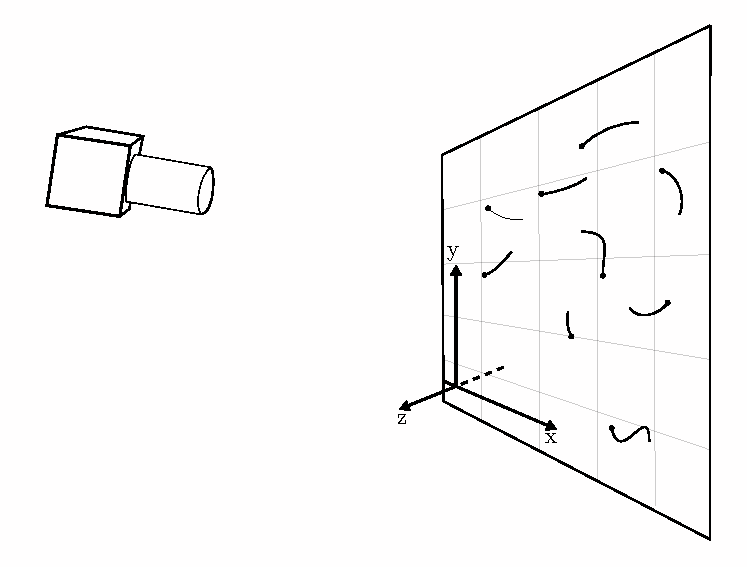
\includegraphics[width=8cm]{2D_tracking_setup.pdf}
	\caption{An example for experimental setup for 2D tracking. Note that the camera doesn't have to be perpendicular to the particles' plane and that the particles don't have to be at $z=0$. \label{fig:2D_tracking}}
\end{figure}


The 2D particle tracking procedure requires following these steps:
%
\begin{enumerate}
	\item Prepare a calibration folder as described in Sec.~\ref{sec:workflow_exp_folder}
	%
	\item Go through camera calibration as shown in Sec.~\ref{sec:cal_guide}
	%
	\item Perform particle segmentation of the particle images, as described in Sec.~\ref{sec:workflow_segment}
	%
	\item Track the particles' coordinates using the workflow script using the \texttt{2D\_tracking} command (see Sec.~\ref{sec:workflow_commands}). The various parameters of the \texttt{params\_file} associated with 2D tracking are given in Tab.~\ref{tab:2d_tracking}
	%
	\item If needed, follow smoothing (Sec.~\ref{sec:workflow_smooth}) and stitching (Sec.~\ref{sec:workflow_stitch}) of the results
\end{enumerate}
%

%
\begin{table}[!ht]
	\centering
	\caption{The \texttt{params\_file.yml} parameters for the 2D tracking step. All paths to files are relative to the \texttt{workflow.py} script. \label{tab:2d_tracking}}
	\begin{tabular}{l m{10cm}}
		\hline
		Parameter & Description\\
		\hline
		
		\texttt{blob\_file} & The name of the file that contains the segmentation results \\
		\texttt{frame\_start} & The number of the first frame from which we want to perform 2D tracking \\
		\texttt{N\_frames} & The number of frames to be analyzed; If \texttt{None}, then all the frames will be analyzed \\
		\texttt{camera\_name} & the name of the camera from which the images were taken (must be a calibrated camera) \\
		\texttt{camera\_resolution} & A tuple representing the camera resolution, for example, (1280, 1024) \\
		\texttt{z\_particles} & The value of the z coordinate of the plane on which the particles are found, e.g. 0.0 \\
		\texttt{d\_max} &  The maximum allowable particle translation between frame in lab-coordinates\\
		\texttt{dv\_max} & The maximum allowable change of velocity for the particles in lab-space coordinates per frame (e.g. mm/frame) \\
		\texttt{save\_name} & The name of the file used to save the results \\
		
		\hline
	\end{tabular}
\end{table}








\clearpage


\section{Imaging module - \texttt{imaging\_mod.py}}\label{sec:image_mod}


The imaging module is used to handle the translation from 2D image space coordinates to lab space coordinates and vice versa through the 3D model. 



\subsection{The \texttt{camera} object}\label{sec:camera}

An object that stores the camera external and internal parameters and handles the projections to and from image space and lab space. Inputs are:

\begin{enumerate}
	\item \texttt{name} - string, name for the camera. This is the name used when saving and loading the camera parameters.
	\item \texttt{resolution} - tuple (2), two integers for the camera number of pixels
	\item \texttt{cal\_points\_fname} - string (optional), path to a file with calibration coordinates for the camera. The format fro the calibration point file is given in Section~\ref{sec:calpointreader} (see Fig.~\ref{fig:calpointfile}).
\end{enumerate}


The important functionality options are:


\begin{enumerate}
	\item \texttt{get\_r(eta, zeta)} - Will solve eq.~\ref{eq:3dmodel} for the orientation vector $\vec{b} = \vec{r} - \vec{O}$, given an input of pixel coordinates $(\eta, \, \zeta)$.
	
	\item \texttt{projection(x)} - Will reverse solve equation~\eqref{eq:3dmodel} to find the image space coordinates $(\eta, \, \zeta)$, of an input 3D point, (\texttt{x=}$\vec{r}$).
	
	\item \texttt{save(dir\_path)} - Will save the camera parameters in a file called after the camera name in the given directory path, see Fig.~\ref{fig:camfiles}.
	
	\item \texttt{load(dir\_path)} - Will load the camera parameters in a file called after the camera name in the given directory path, see Fig.~\ref{fig:camfiles}.
\end{enumerate}



After calibration we can save the camera parameters on the hard disc. The camera files have the structure shown in Fig.~\ref{fig:camfiles}.

\begin{figure}[!ht]
	\centering
	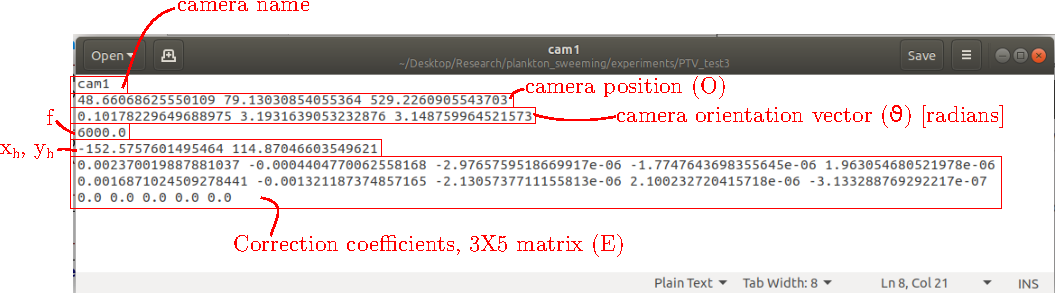
\includegraphics[width=\textwidth]{camera_files.pdf}
	\caption{The structure of a camera file. The files are simple text files where each row corresponds to a specific parameter and the values in each row are separated by a white space. \label{fig:camfiles}}
\end{figure}








\subsection{The \texttt{imsys} object}


An object that holds several camera instances and can be used to perform stereo-matching. The important functionalities are:


\begin{enumerate}
	\item \texttt{stereo\_match(coords, d\_max)} - Takes as an input a dictionary with coordinates in image space from the several cameras and calculates the triangulation position. \\ The coordinate dictionary has keys that are the camera number and the values which are the coordinates in each camera. d\_max is maximum allowable distance for the triangulation.
	
\end{enumerate}








\subsection{The \texttt{Cal\_image\_coord} object}\label{sec:calpointreader}

This is a class used for reading information given in the optional argument \texttt{cal\_points\_fname} of the \texttt{camera} class (Sec.~\ref{sec:camera}). It is used internally and generally users will not have to deal with this. This class will read and interpret text files with tab separated valued, where the columns' meanings are: [x image space, y image space, x lab space, y lab space, z lab space], and each row is a single point of some known calibration target.

The input for this class is:
\begin{enumerate}
	\item \texttt{fname} - String, the path to your calibration point file. The file is holds tab separated values with the meaning of: [x image, y image, x lab, y lab, z lab], see Fig.~\ref{fig:calpointfile}.
\end{enumerate}








\section{Camera calibration - \texttt{calibrate\_mod.py}}


The \texttt{calibrate\_mod.py} module, with the \texttt{calibrate} object, is used to find the camera calibration parameters. We calibrate each camera by taking an image of a \textit{calibration target} - a body with markings of known coordinates in lab space - and search for the camera parameters that minimize the distance between the projection of the known points in image space and the image taken with the camera. In addition to that, after a calibration is made and trajectories have been obtained, the calibration might be refined by using the \texttt{calibrate\_with\_particles} object; this is particularly helpfull in cases where some of the cameras slightly moved in between the taking the calibration images and the recording of the tracer particles.



\subsection{The \texttt{calibrate} object}\label{sec:calibrate_obj}

Used to solve for the camera parameters given an input list of image space and lab space coordinates. The inputs are:

\begin{enumerate}
	\item \texttt{camera} - An instance of a \texttt{camera} object which we would like to calibrate.
	\item \texttt{lab\_coords} - a list of lab space coordinates of some known calibration target. 
	\item \texttt{img\_coords} - a list of image space coordinates that is ordered in accordance with the lab space coordinates. 
\end{enumerate}



The important functionalities are:
%
\begin{enumerate}
	
	\item \texttt{searchCalibration(maxiter=5000, fix\_f=True)} - When this is run, we use a nonlinear least squares search to find the camera parameters that minimize the cost function (item 3 below). This function is used to find the $\vec{O}$, $\vec{\theta}$, $f$, and $x_h, \, y_h$ parameters (in case \texttt{fix\_f=False}, it will not solve for $f$. \texttt{maxiter} is the maximum number of iterations allowed for the least squares search.
	
	\item \texttt{fineCalibration(maxiter=500)} - This function will solve for the coefficients of the quadratic polynomial used for the nonlinear correction term ($[E]$). 
	
	\item \texttt{mean\_squared\_err} - This is our cost function, being the sum of distances between the image space coordinates and the projection of the given lab space coordinates.
	
\end{enumerate}
%
To find an optimal calibration solution, we might need to run each function several times, and run the coarse and fine calibrations one after the other until a satisfactory solution is obtained. Once it is obtained, we should keep in mind to save the results using the \texttt{save} functionality of the \texttt{camera} object. 





\subsection{The \texttt{calibrate\_with\_particles} object}\label{sec:calibrate_with_particles_obj}

A class used to refine the calibration using particles data. In short,
after the primary clibration is done, matching and tracking can be used
to obtain trajectories from the experimental data. Assuming that this resulted in trajectories that were successfully measured, we can leverage
the trajectories obtained to minimize further the calibration error. The refinement is done by assuming that the positions of particles along the resolved trajectories are "true" positions in lab-space, and thus, the blobs corresponding to these particles are used in a calibration sequence to minimize the calibration error. The assumption is that longer trajectories with low triangulation error are considered more reliable as compared to shorter trajectories, so we use only "long enough" trajectories 
in this process.

The inputs are:

\begin{enumerate}
	\item \texttt{traj\_filename} - the name of the file containing the trajectories from
	which the calibration points are taken.
	
	\item \texttt{camera} - an instance of the camera we wish to try and re-calibrate
	
	\item \texttt{cam\_number} - int, >= 1; the number (index) of the camera to be
	calibrated. For example, to calibrate camera2, this should be set to 2.
	
	\item \texttt{blobs\_fname} - The name of the file that contains the segmented 
	particles' data.
	
	\item \texttt{min\_traj\_len} - Only trajectories longer then this number will be used in the calibration
	
	\item \texttt{max\_point\_number} - the maximum number of points that shall be taken
	to re-calibrate the camera. Note that too many points (say above 1000) might lead to long calculation times. 
\end{enumerate}


The important functionalities are:

\begin{enumerate}
	
	\item \texttt{get\_calibrate\_instance} - This function returns an instance of the \texttt{calibrate} object with the calibration points taken from the trajectory file. We then use this object to refine the calibration using the regular procedure (Sec.~\ref{sec:calibrate_obj}).

\end{enumerate}





\subsection{The \texttt{gui\_final\_cal.py} file}

The \texttt{gui\_final\_cal.py} script is used to launch a \texttt{tkinter} based graphical user interface that is utilized to run various functionalities of the calibration process. The GUI is shown in  Fig.~\ref{fig:calibration_gui}, and the various buttons are explained in Tab.~\ref{tab:calibration_gui}.




\subsection{The \texttt{gui\_initial\_cal.py} file}

The \texttt{gui\_initial\_cal.py} script is used to launch a \texttt{tkinter} based graphical user interface that is utilized to run various functionalities of the calibration process. The GUI is shown in  Fig.~\ref{fig:init_cal_gui} and it is explained in section~\ref{sec:init_calibration}.












\section{Particle segmentation - \texttt{segmentation\_mod.py}} 


This module handles the image analysis part of MyPTV, taking in raw camera images containing particles and output their image space coordinates. For the segmentation we first blur the image to remove salt and pepper noise, then we highlight particles using a local mean subtraction around each pixel, and then use a global threshold to mark foreground and  pixels. Finally, the connected foreground pixels are considered to be particles, and we estimate the blob's center using a brightness weighted average of blob pixels.



\subsection{The \texttt{particle\_segmentation} object} 

Used to segment particles in a given image. This class is used internally to iterate over frames in a single folder by the \texttt{loop\_segmentation} class. However, it is recommended to check the segmentation parameters manually using this \texttt{particle\_segmentation} over several images in order to tune the particle searching parameters. The inputs are:
%
\begin{enumerate}
	\item \texttt{image} - the image for segmentation
	\item \texttt{threshold=10} - the global filter's threshold brightness value, so pixels with brightness higher than this number are considered foreground 
	\item \texttt{mask=1.0} - A mask matrix can be used to specify rigions of interest within the image
	\item \texttt{sigma=None} - If float, this is taken as the standard deviation of a Gaussian blurring filter; if it is None, no bluring is performed
	\item \texttt{median=None} - If integer this is taken as the window size for a median noise removal filter; if None, no median filter is performed
	\item \texttt{local\_filter=None} - Parameters for a local mean subtraction. If it's an interger it is taken as the window size; is it None, no mean subtraction is performed.
	\item a bunch of threshold pixel sizes and mass in all directions and in area.
	\item \texttt{method} - String. The name of the method used for segmentation (either 'labeling' or 'dilation', see Sec.~\ref{sec:workflow_segment}). Default is 'labeling'.
	\item \texttt{particle\_size=3} - The particle size used in the dilation method.
\end{enumerate}


The important funcitonalities are:
%
\begin{enumerate}
	\item \texttt{get\_blobs} - Will return a list of blob centers, their box size and their area.
	
	\item \texttt{plot\_blobs()} - Uses matplotlib to plot the results of the segmentation. A very useful functionality in the testing of segmentation parameters!
	
	\item \texttt{save\_results(fname)} - Will save the segmented particles in a text file. The file is arranged in six columns with the following attributes: (x center position, y center position, x size, y size, area, image number), see Fig.~\ref{fig:blobfile}.
\end{enumerate}






\subsection{The \texttt{loop\_segmentation} object} 


An object used for looping over images in a given directory to segment particles and save the results in a file. The inputs are nearly identical to those of \texttt{particle\_segmentation}.


important functionalities are:
%
\begin{enumerate}
	\item \texttt{segment\_folder\_images()} - Will loop over the images in the given directory and segment particles according to the given parameters
	\item \texttt{save\_results(fname)} - Will save the segmented particles in a text file. The file is arranged in six columns with the following attributes: (x center position, y center position, x size, y size, area, image number), see Fig.~\ref{fig:blobfile}.
\end{enumerate}

\begin{figure}[!ht]
	\centering
	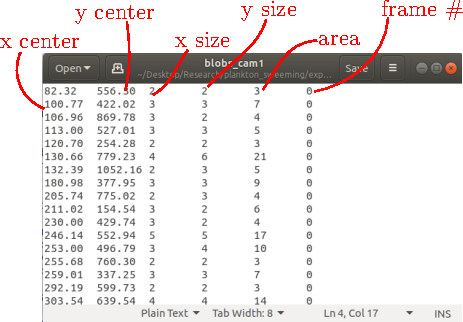
\includegraphics[width=10cm]{blob_file.pdf}
	\caption{An example of a text file holding the segmentation resuls and the description of the different columns. \label{fig:blobfile}} 
\end{figure}








\section{Particle matching - \texttt{particle\_matching\_mod.py}} \label{sec:matching}

The module used to link particles in the different images through stereo matching and estimating their 3D positions. One of the main issue in this process is that stereo matching all possible candidates is an NP hard problem, so to track numerous particles in each frame we have to choose which particles are likely to produce a 3D particle coordinate. Thus, particle matching in MyPTV uses two algorithms in conjunction. First is a novel algorithm that uses 2D time tracking of blobs to deduce which candidates are more likely to produce traceable particles in 3D. Second is the Ray Traversal algorithm proposed in Ref~\cite{Bourgoin2020}, in which the lab space volume is divided to voxels and stereo matching is attempted for rays within each voxel. Using the two algorithms in conjunction was found to yield a 50\% reduction in computational time and more traceable trajectories (45\% more trajectories were found in a test). 




\subsection{The \texttt{match\_blob\_files} object}


This is the object that we use to get triangulated particles results from the segmented blob files (a file as the one in Fig.~\ref{fig:blobfile} for each camera). For each frame it first runs the first algorithm using time information, and only then uses the Ray traversal algorithm on the blobs that were not successfully connected. The inputs are:
%
\begin{enumerate}
	\item \texttt{blob\_fnames} - a list of the (srting) file names containing the segmented blob data. The list has to be sorted according the order of cameras in the \texttt{img\_system}.
	
	\item \texttt{img\_system} - an instance of the \texttt{img\_system} class with the calibrated cameras.
	
	\item \texttt{RIO} - A nested list of 3X2 elements. The first holds the minimum and  maximum values of $x$ coordinates, the second is same for $y$, and  the third for $z$ coordinates. 
	
	\item \texttt{voxel\_size} - the side length of voxel cubes used in the ray traversal algorithm. Given in lab space coordinates (e.g. mm). Note - a too large voxel size will result in high computational times due a high number of candidates, while a too small voxel size might lead to erroneous intersection of rays, leading to matching errors. Thus, this parameter should be optimized.
	
	\item \texttt{max\_blob\_dist} - the largest distance for which blobs are considered neighbours in the image space coordinates (namely, the largest permissible blob displacement in pixels).
	
	\item \texttt{max\_err=None} - Maximum acceptable uncertainty in particle position. If None, (defult), than no bound is used.
	
	\item \texttt{reverse\_eta\_zeta=False} - Should be false if the eta and zeta coordinates need to be in reverse order so as to match the calibration. This may be needed if the calibration data points were given where the x and y coordinates are transposed (as happens, e.g., if using matplotlib.pyplot.imshow).
\end{enumerate}


The important functionalities are:
%
\begin{enumerate}
	\item \texttt{get\_particles()} - Use this to match blobs into particles in 3D.
	\item \texttt{save\_results(fname)} - Save the results in a text file. The format has 4 + number of cameras columns separated by tabs:
	(x, y, z, [N columns corresponding to the blob number in each camera] , frame number, see Fig.~\ref{fig:particlefile}).
\end{enumerate}



\begin{figure}[!ht]
	\centering
	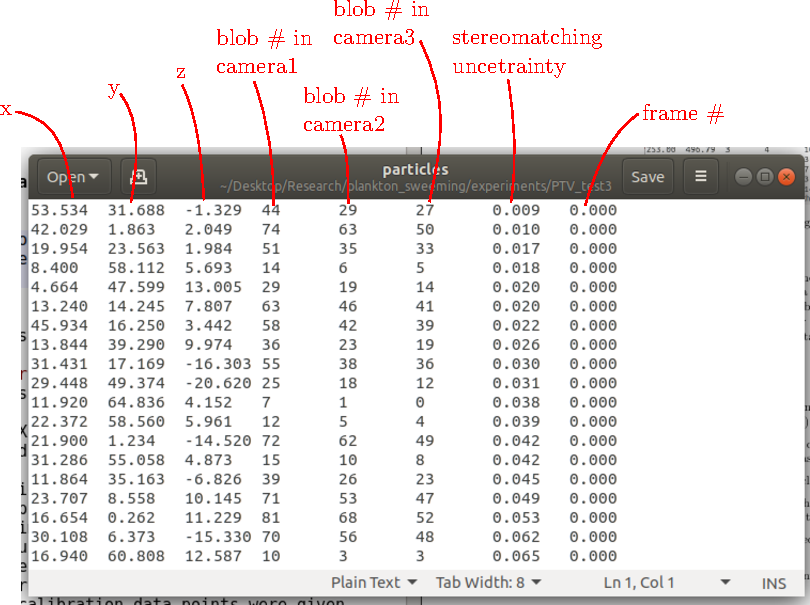
\includegraphics[width=12cm]{particle_file.pdf}
	\caption{An example of a text file holding the triangulated particles' resuls and the description of the different columns. In this example there were three cameras. The blob number columns give the index of the blobs corresponding to any particle at the this specific frame number; a value of -1 in one of the rows means that no blob was used to stereo-match the particle in this row for this particular camera. \label{fig:particlefile}} 
\end{figure}




\subsection{The \texttt{matching} object}

This object is the "engine" used to match particles using the Ray Traversal algorithm. In practice we run the relevant functions: \texttt{get\_voxel\_dictionary()} $\rightarrow$ \texttt{list\_candidates()} $\rightarrow$ \texttt{get\_particles()}, and after that the results are held in the attribute \texttt{matched\_particles}.




\subsection{The \texttt{matching\_using\_time} object}

This object performs the matching of blobs using the 2D tracking heuristic. In principle, it is given a list of blobs that were successfully used to form 3D particles in the previous frame. Then, for each of the given blobs it searches for nearest neighbours in the current frame, and stereo-matches those blobs that were found (using the \texttt{.triangulate\_candidates()} method). 





\subsection{The \texttt{initiate\_time\_matching} object}

This object is used to initiate the time searching algorithm on the first frame. It goes over the blobs at the first frame and searches for blobs that have nearest neighbours at the second frame. Those that have neighbours are used in a first run of the Ray Traversal algorithm, thus they are given priority in the search.













\section{Tracking in 3D - \texttt{tracking\_mod.py}}

This is the module that is used to track particles in 3D. There are currently three tracking methods implemented, nearest neighbour, two-frame, and four-frame, see Ref.~\cite{Ouellette2006}. Users are welcome to choose their preferred method and use it.



\subsection{The \texttt{tracker\_four\_frames} object}\label{sec:four_frames}

An object used to perform tracking through the 4-frame best estimate method \cite{Ouellette2006}. Input:
%
\begin{enumerate}
	\item \texttt{fname} - a string name of a particle file (e.g. Fig.~\ref{fig:particlefile}
	\item \texttt{mean\_flow=0.0} - either zero (default) of a numpy array of the mean flow vector, in units of the calibrations spatial units per frame (e.g. mm per frame). The mean flow is assumed not to change in space and time.
	\item \texttt{d\_max\_=1e10} - maximum allowable translation between two frames for the nearest neighbour search, after subtracting the mean flow. 
	\item \texttt{dv\_max\_=1e10} - maximum allowable change in velocity for the two-frame velocity projection search. The radius around the projection is therefore dv\_max/dt (where dt = 1 frame$^{-1}$)
\end{enumerate}


The important functionality is:
%
\begin{enumerate}
	\item \texttt{track\_all\_frames()} - Will track particles through all the frames. 
	
	\item \texttt{return\_connected\_particles()} - Will retun the list of trajectories that were established.
	
	\item \texttt{save\_results(fname)} - Will save the results on the hard drive. The results are saved in a text file, where each row is a sample of a trajectory. The columns are specified as follows: [trajectory number, x, y, z, frame number], see Fig~\ref{fig:trajfile}.  
\end{enumerate}

\begin{figure}
	\centering
	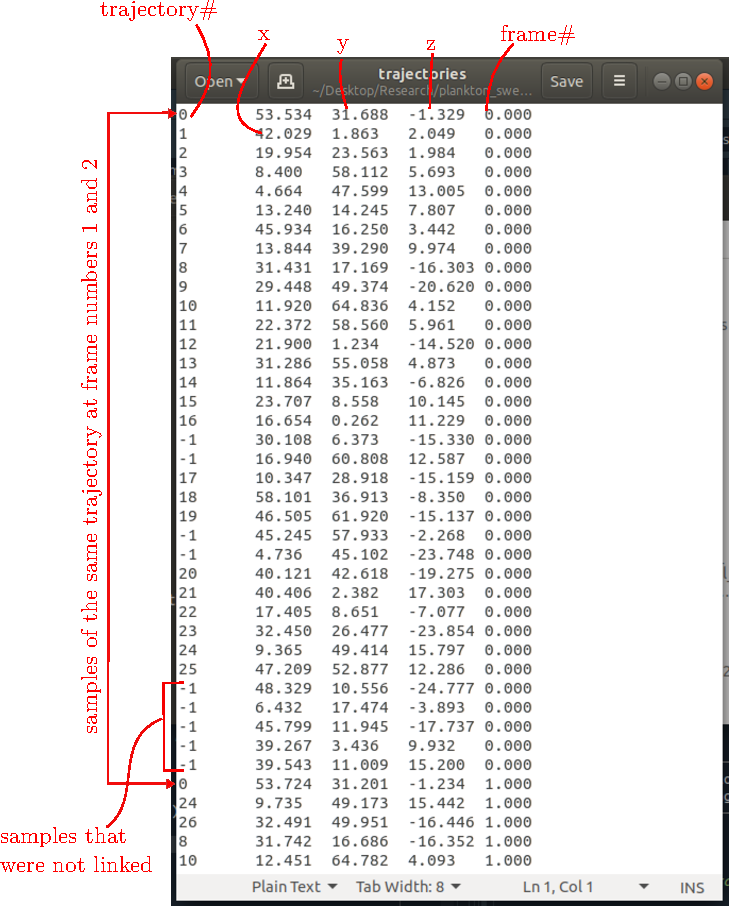
\includegraphics[width=10cm]{trajectory_files.pdf}
	\caption{Example of a trajectory file and the column definitions. For Trajectory id being a non-negative integer, rows with the same Trajectory id correspond to the same trajectory; rows with Trajectory id being -1 are samples that could not be linked with the given tracking parameters.  \label{fig:trajfile}}
\end{figure}




\subsection{The \texttt{tracker\_two\_frames} object}

An object used for tracking through the 2-frame method. The description is the same as in Section~\ref{sec:four_frames}



\subsection{The \texttt{tracker\_nearest\_neighbour} object}

An object used for tracking through the nearest neighbour method. The description is the same as in Section~\ref{sec:four_frames}









\section{Trajectory smoothing - \texttt{traj\_smoothing\_mod.py}}

This module is used to smooth trajectories and to calculate the velocity and acceleration of the particles. For the smoothing we are using the polynomial fitting method proposed and used in Refs.~\cite{Luthi2005, Shnapp2019}. In short, each component of the particle's position is fitted with a series of polynomials with a sliding window of fixed  and the derivatives are calculated by analytically differentiating the polynomial. The end result is a new file with smoothed trajectories. However note that we smooth and calculate velocities and accelerations only for trajectories longer than the window size for the smoothing (a user decided parameter). 


\subsection{The \texttt{smooth\_trajectories} object}

A class used to smooth trajectories in a list of trajectories. Due to the smoothing we also calculate the velocity and acceleration of the trajectories. The input trajectory list structure is the same as the files produced by the classes in \texttt{tracking\_mod.py}.

Note - only trajectories whose length is larger than the window size will be smoothed and saved. Shorter trajectories are saved with zero velocity and accelerations.


The inputs are:
\begin{enumerate}
	\item \texttt{traj\_list} -  a list of samples organized as trajectories. This should have the same data structure used in the saving function of the tracking algorithms (see Section~\ref{sec:four_frames}). 
	\item \texttt{window} - The window size used in the sliding polynomial fitting.
	\item \texttt{polyorder} - The order of the polynomial used in the fitting. 
\end{enumerate}

\begin{figure}[!ht]
	\centering
	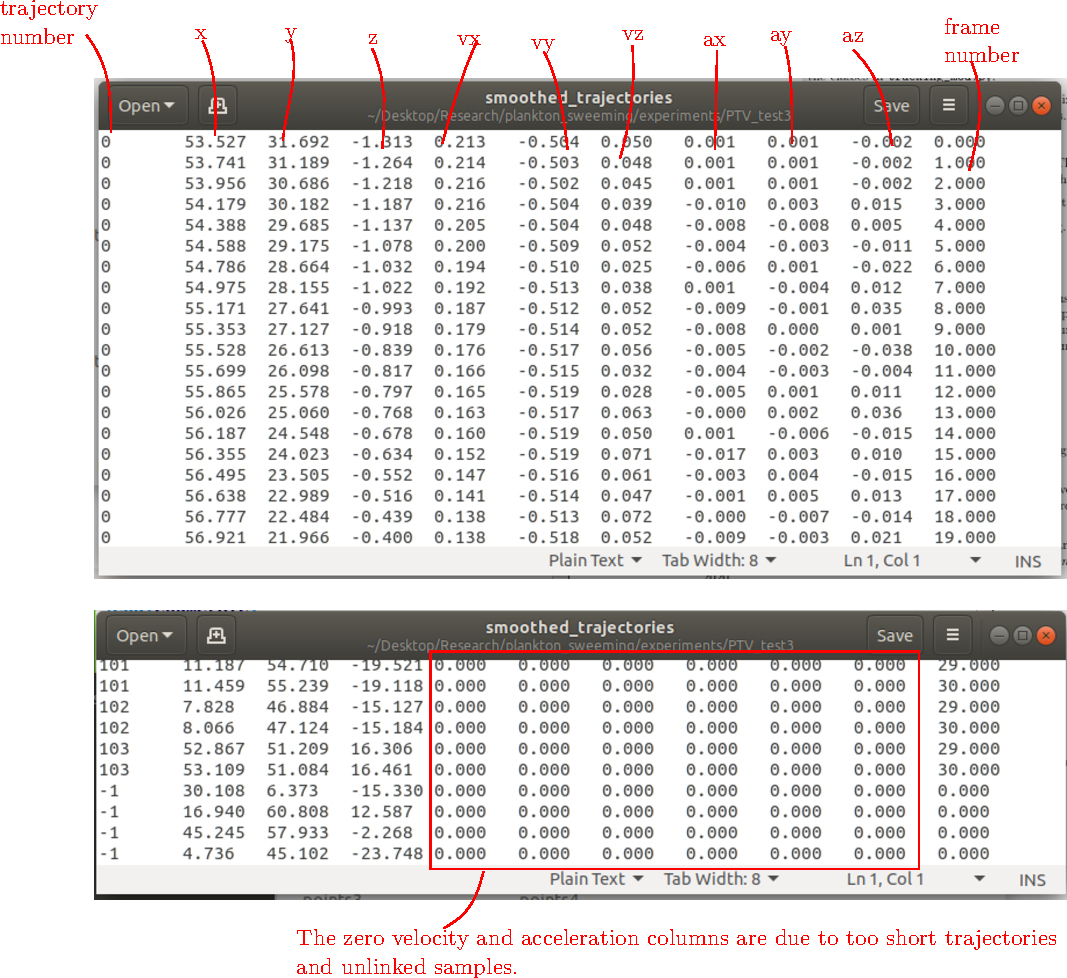
\includegraphics[width=12cm]{smoothed_trajfile.pdf}
	\caption{Example file holding the results of smoothed trajectories, and the description for each column. Note also the unsmoothed samples at the bottom of the file. \label{fig:smoothedfile}}
\end{figure}

The important functionality is:

\begin{enumerate}
	\item \texttt{smooth()} - performs the actual smoothing
	\item \texttt{save\_results(fname)} - Saves the results on the hard drive using the given (string) file name. The resulting file is a text file such that each row is a sample of a trajectory, and with 11 columns. The columns have the following meaning:
	[traj number, $x$, $y$, $z$, $v_x$, $v_y$, $v_z$, $a_x$, $a_y$, $a_z$, frame number], where $v_i$ and $a_i$ denote components of the velocity and acceleration vectors respectively, see Fig.~\ref{fig:smoothedfile}.
\end{enumerate}







\section{Trajectory stitching - \texttt{traj\_stitching\_mod.py}}\label{sec:stitching}

This module applies the algorithm by Ref.~\cite{Xu2008} to connect trajectories that were broken along the process by tracking the trajectories again in the position--velocity space. We also extend this by interpolating the missing samples using a 3rd order polynomial, that is fitted to the existing 4 data points at the tips of the broken trajectories. This module is applied after the trajectory smoothing step.




\subsection{The \texttt{traj\_stitching} object}

This object performs the stitching process. Inputs:

\begin{enumerate}
	\item \texttt{traj\_list} - the list of smoothed trajectory, given as a Numpy array of shape (N,11), where N is the number of samples. The format is the same as the format generated after the smoothing process.
	\item \texttt{Ts} - The maximum number of broken samples allowed in the connection.
	\item \texttt{dm} - The maximum distance between the trajectory for which connections are made.
\end{enumerate}



The important functionalities are:

\begin{enumerate}
	\item \texttt{stitch\_trajectories()} - Will search for candidates and stitch the best fitting candidates. Run this function to perform the stitching. After running the new trajectory list is held as the attribute \texttt{new\_traj\_list}.
	
	\item \texttt{save\_results(fname)} - Will save the stitched trajectories in a text file with a given file name. The format for the saved file is the same as the one used in the smoothing trajectories (Fig.~\ref{fig:smoothedfile}).
\end{enumerate}





\bibliography{bib_myPTV}
\bibliographystyle{unsrt}

\end{document}